\chapter{低驱动电压硅基混合集成III-V电吸收光调制器}
基于QCSE效应的电吸收光调制器具有高速,低能耗,高消光比和小尺寸的特别点\cite{tang2012energy, fukano2006very}。因此电吸收光调制器被广泛应用于光通信领域。另外,电吸收光调制器具有双工作模,还可以被用于高速的光探测器\cite{welstand1996dual}。基于这个特性,研究人员实现了光电振荡器(Optoelectronic Oscillators, OEO)\cite{zhou2014compact}。我们最近也实现了单片集成的光收发器\cite{chen2016wavelength}。最近,由于硅光子和晶体管可以在统一的半导体工艺线上制作。这给复杂的光电集成系统,比如集成光子微波系统\cite{Marpaung2013integrated}和芯片间的光互联系统\cite{sun2015single},带来了希望。基于硅和III-V的键合技术,已经实现硅基混合集成III-V光调制器\cite{kuo2008high,tang201150,tang2012over,tang2012energy,chen2011forty,Srinivasan2012micro,fu20155}。不过,硅基光芯片中,低能耗是十分重要的指标。又因为电吸收光调制器的驱动电压与能耗成平方关系,见公式\ref{Equ:EC}。因此,硅基光芯片中低驱动电压的光调制器十分重要。另外,如果电吸收光调制器能够直接被来自逻辑电路的低电压信号驱动,那么消耗于电的放大器的能量也会被节省下来。最近,研究人员们在纯硅上展示了100~mV以下的硅基光调制器,见表格\ref{sil_mod}。然而,这些硅的调制器都是基于光的谐振腔结构,见图\ref{fig_mod_opt_type}(a)所示,它们对工艺的要求十分苛刻,并且还不能用于光探测器。对于传统的基于QCSE的电吸收光调制器,降低驱动电压的同时保持同样的尺寸和插入损耗十分困难。尽管研究人员利用复杂的基于慢光效应的布拉格波导\cite{gulow-voltage2013},降低了电吸收光调制器的驱动电压,但是这种结构的光调制器不仅无法和硅光子器件集成也无法将驱动电压降低到硅调制器的层次。因此,我们需要寻找一种新的思路实现低驱动电压的光调制器。

本章概述了基于能带填充效应的新型低驱动电吸收光调制器,首先介绍了低驱动电压电吸收光调制器的原理。接着阐述了设计和和仿真结果。然后,详细介绍了制作调制器的步骤。最后,在搭建的高速光调制器测试平台上,对低驱动电压光调制器的性能进行了测试。
\section{低驱动电压光调制器的原理}
\begin{figure}[htb]
	\centering
	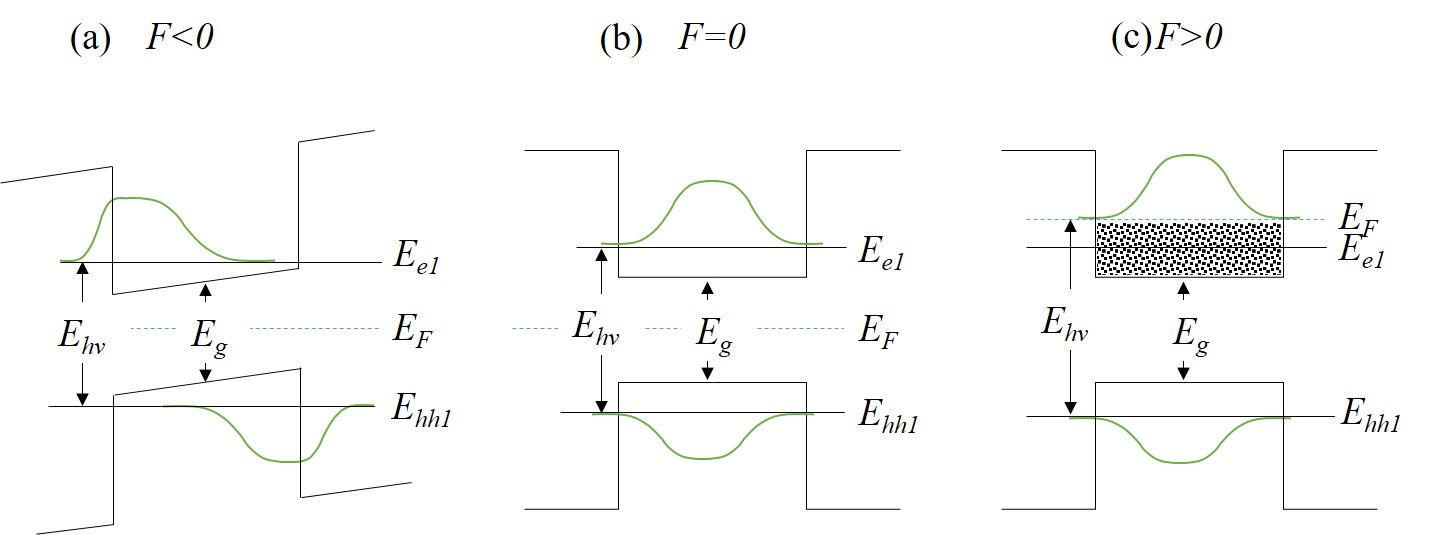
\includegraphics[width=14cm]{./Pictures/fig_ch4_bandfilling_diag.jpg}
	\caption{ 量子阱的能带和波函数的示意图(a)有外界反向电场下;(b)在外界无电场的时候;(c)在外界正向电子子注入的时候}
	\label{fig_ch4_band_lineup}
\end{figure}
调制掺杂中的多量子阱 (Modulation-doped Multiple Quantum-wells) 中的能带填充效应在80年代已经被深入研究\cite{livescu1988free}。能带填充效应与QCSE效应的原理示意图见图\ref{fig_ch4_band_lineup}。当正向电子注入多量子阱中势阱的导带时,相应的电子准费米能级就被提高。当电子的准费米能级高过导带中最低的能级时,即最低的能级被二维电子气体填充慢时,导致了原本激子吸收峰对应的光子无法被吸收,因此其产生的电子无法跃迁到最低的能级处。这意味着只有更高能量的光子才会被吸收,使产生电子跃迁到准费米能级处。可以预测随着注入电子浓度的增加,使电子的准费米能级逐渐升高,导致了激子吸收峰的蓝移。除此之外,根据公式\ref{Equ:excitonabs}所示,激子吸收峰的强度与电子空穴波函数的重叠积分成平方关系。基于QCSE效应,外加的电场会使能带结构倾斜,从而电子空穴的重叠积分减弱,如图\ref{fig_ch4_band_lineup}(a)所示,导致激子吸收峰随着外界电场的增强而减弱,见图\ref{fig_ch2_te_abs}。而基于能带填充效应,由于能带结构并不会发生明显变化(只会由于电子间的多体效应导致能带结构发生微弱的形变\cite{livescu1988free}),电子和载流子的波函数与无外界电场下的波函数几乎相同,如图\ref{fig_ch4_band_lineup}(c)所示。因此激子吸收峰的强度随着电子浓度的增加而将保持一致。这为实现低驱动电压的电吸收光调制器提供了条件。

激子吸收峰对应光子能量的漂移量$\Delta E$与电子准费米能级$E_F$的关系如下式所示\cite{livescu1988free}:
\begin{equation}
\label{Equ:DEEF}
\Delta E = (1+m_e/m_h)E_F,
\end{equation}
其中$m_e$和$m_h$分别是电子和空穴的等效质量。当$E_F$远大于导带中最低的能级$E_1$时,电子的准费米能级和量子阱中载流子浓度成线性关系,见公式\ref{Equ:E1EF}\cite{coldren1995diode}。
\begin{equation}
\label{Equ:E1EF}
E_F = \pi\hbar^2d_xN/m_e+E_1,
\end{equation}
其中$d_x$是多量子阱中所有势阱的宽度。我们可以通过控制偏置电压,调节注入电流,从而调节量子阱区域的电子浓度。电流与载流子浓度的关系见公式\ref{Equ:VN}。
\begin{equation}
\label{Equ:VN}
N = \frac{\tau\eta I}{qV}
\end{equation}
其中,$\tau$是载流子寿命,$\eta$是载流子注入效率,I是注入电流,V是调制器有源区体积,q是电子的基本电荷。因此,利用能带填充效应,多量子阱的激子吸收峰的位置就可以通过偏置电压来控制。利用调制掺杂的多量子阱中的能带填充效应,已经被应用于只需要100 mV驱动电压的Q调制器的激光器\cite{kalinovsky1993free}。而我们在此展示的低驱动电压的电吸收光调制器是首个基于能带填充效应的光调制器。

\section{调制器的设计与仿真}
考虑到电子束光刻制作III-V波导与硅波导的耦合结构比较困难。我们设计的低驱动电压的硅基混合集成III-V电吸收光调制器将采用普通的接触式光刻工艺制作,并且为了降低工艺成本,波导加工将采用纯湿法腐蚀。因此,我们将采用蘑菇型的波导结构。波导截面结构示意图,如图\ref{chapt4_structure_mode_profile}(a)所示。硅波导的结构是380 nm厚,刻蚀深度160 nm的脊型波导。并且表面利用SiO\SB{2}进行平坦化。上面是利用DVS-BCB和SiO\SB{2}的键合层。再往上是III-V结构,与图\ref{fig_ch2_banddiagram}(a)相同。具体结构的组分如表\ref{epi_material},各个组分的材料参数,比如折射率等,见表\ref{epi_structure}。
{
	\begin{table}[htb]
		\zihao{5}
		\caption{III-V 波导的材料参数。$\lambda_{ex}$:激子吸收峰波长}
		\label{epi_material}
		\centering
		\begin{tabular}[t]{llll}
			\hline
			名称 & 材料组分 & 掺杂浓度 (cm\SP{-3}) & 厚度 \\
			\hline
			p-contact &In\SB{0.53}Ga{0.47}As& p-1.5$\times$10\SP{19}& 0.1$\mu m$  \\ 
			\hline
			p-cladding  & InP & p-2$\times$10\SP{18} to p-1$\times$10\SP{18} &1.5 $\mu m$ \\
			\hline
			SCH & In\SB{0.52}Al\SB{0.16}Ga\SB{0.32}As& - &0.15 \\
			\hline
			\multirow{2}{*}{\tabincell{l}{MQW \\ ($\lambda_{ex} = 1560~nm$)}}
			& Well:~In\SB{0.65}Al\SB{0.09}Ga\SB{0.26}As,(10$\times$) & -& 110~nm\\ 
			\cline{2-4} 
			&Barrier:~In\SB{0.42}Al\SB{0.17}Ga\SB{0.39}As,(11$\times$) &-& 70~nm\\
			\hline
			SCH & In\SB{0.52}Al\SB{0.16}Ga\SB{0.32}As& - & 0.1 $\mu m$\\
			\hline
			n-contact & InP& n-3$\times$10\SP{18} & 0.15 $\mu m$ \\
			\hline
		\end{tabular}
	\end{table}
}

\begin{figure}[htb]
	\centering
	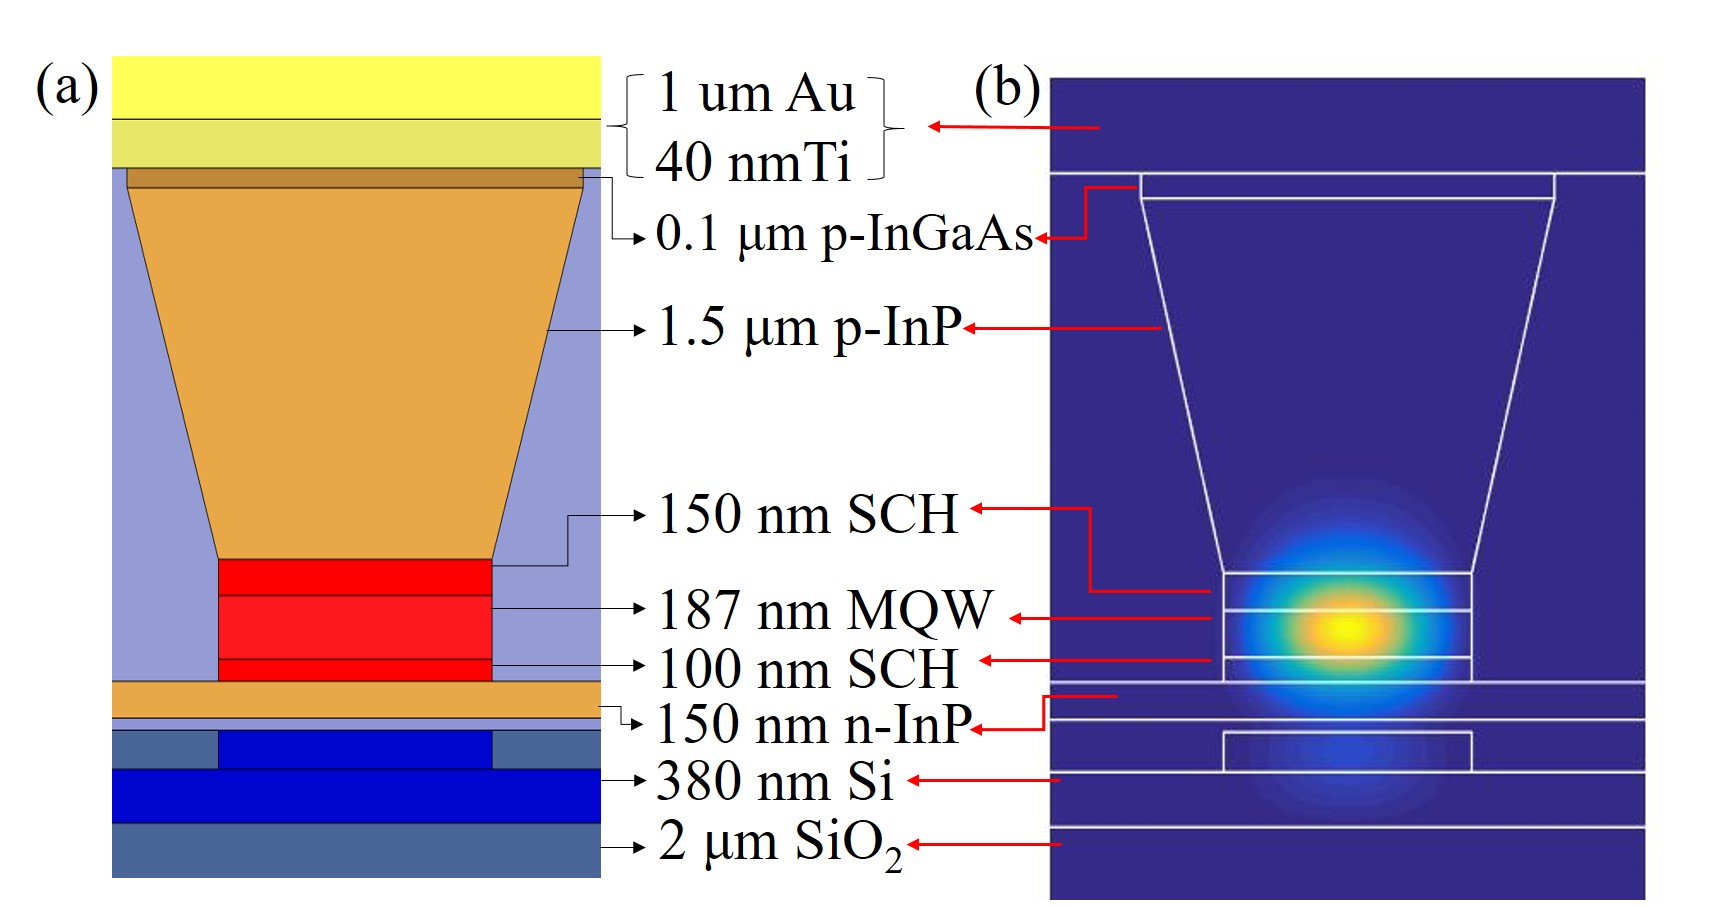
\includegraphics[width=14cm]{./Pictures/chapt4_structure_mode_profile.jpg}
	\caption{ (a)硅基混合集成III-V调制器的截面图;(b)硅基混合集成III-V调制器波导的基模电场强度图}
	\label{chapt4_structure_mode_profile}
\end{figure}

在波导宽度方面设计,考虑到接触式光刻的精度最小$1~\mu m$左右,我们将多量子阱区域的波导宽度设计为$1.5~\mu m$。此时光场在10层势阱中的限制因子大概达到24\%。模场分布图见图\ref{chapt4_structure_mode_profile}(b)所示。图中p-InP之所形成倒梯形,是由于湿法腐蚀各项异性导致的。如果p-InP波导的底部宽度为$1.5~\mu m$,那么$1.5~\mu m$厚的p-InP顶部就有$2.5~\mu m$的宽度。

在电极方面的设计,根据之前小结\ref{electrostructure}对四种不同电极所需驱动电压的分析,我们采用了所需驱动电压最小的集总电极结构。我们设计n电极与波导边缘的间距为$3\mu m$,之所以选择这个偏大的距离,是为了降低对套刻精度的要求,防止金属引起额外吸收损耗。p电极的宽度我们设计为$6 \mu m$。最后,我们根据测试所需探针为GSG (Ground Signal Ground)的针间距为$50~\mu m$,设计了完整的电极结构,如图\ref{chapt4_3D_structure}所示。

\begin{figure}[htb]
	\centering
	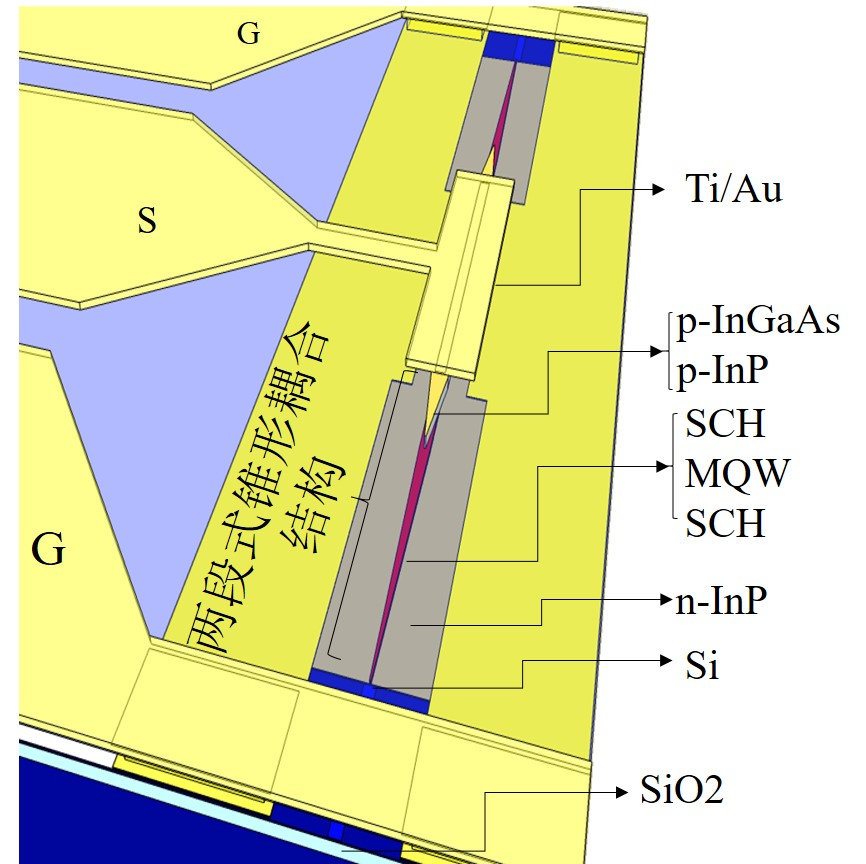
\includegraphics[width=12cm]{./Pictures/chapt4_3D_structure.jpg}
	\caption{ 硅基混合集成III-V电吸收光调制器,采用集总电极的三维结构示意图}
	\label{chapt4_3D_structure}
\end{figure}

在硅波导和混合集成III-V波导的耦合结构中,我们设计的目标是为了减小工艺的难度,并且增加对加工误差的容忍度。因此通过延长了原来的三段使锥形的耦合结构到$45~\mu m$,将第一段和第二段结构合并,使三段式锥形耦合结构简化到两段式耦合结构。同时取消硅波导上的锥形结构,在III-V波导下面硅波导保持$1.5~\mu m$的宽度。这种结构对加工误差的容忍度增大,让沿波导方向的套刻精度需求下降到最低,甚至在改变III-V的结构或者位置时,不需要再改变硅的结构。在具体的设计参数中,第一段锥形耦合结构的长度是$30~\mu m$,其中n-contact层的宽度保持不变,而MQW层和SCH层的宽度从$0.2~\mu m$线性变化到$1.5 ~\mu m$。而第二段锥形耦合结构的长度是$15~\mu m$,其中MQW层和SCH层的宽度保持$1.5~\mu m$的宽度,而p-cladding层和p-contact层的宽度从$0.2~\mu m$逐渐变化到$2.5~\mu m$。整个器件的示意图见图\ref{chapt4_3D_structure}。它在$1.55~\mu m$波长的耦合效率达到了98\%,硅波导和硅基III-V混合集成III-V波导的模式耦合图,如图\ref{chapt4_taper_performance}(a)所示。
\begin{figure}[h]
	\centering
	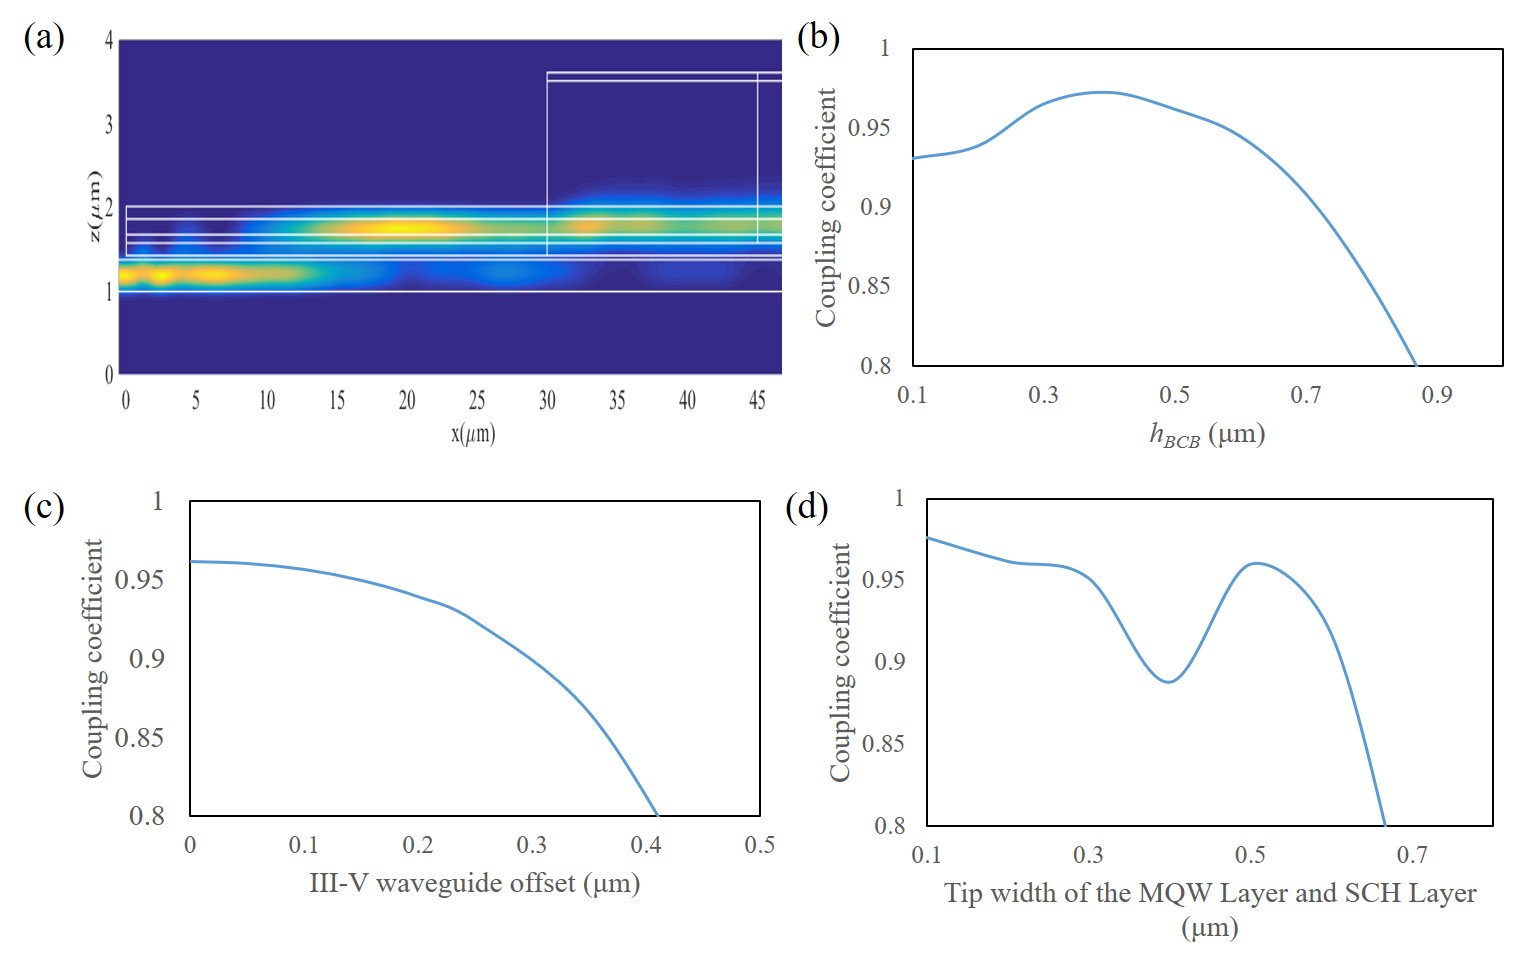
\includegraphics[width=14cm]{./Pictures/chapt4_taper_performance.jpg}
	\caption{两段式锥形耦合结构在$1.55~\mu m$处的分析:(a)光的模场传播图;(b)键合厚度$h_{BCB}$对耦合效率的影响;(c) III-V波导和硅波导的垂直波导方向的套刻误差对耦合性能的影响;(d) MQW层和SCH层锥形尖端宽度对耦合效率的影响}
	\label{chapt4_taper_performance}
\end{figure}

接下来,我们分析这种结构对工艺误差的容忍度,包含了键合层的厚度$h_{BCB}$,III-V波导和硅波导在垂直波导方向的套刻误差,以及MQW层和SCH层锥形尖端宽度对耦合效率的影响,见图\ref{chapt4_taper_performance}(b-d)所示。可以看到当$h_{BCB} < 70 ~nm$时,耦合效率都有90\%以上。当III-V波导和硅波导垂直波导方向的套刻偏差小于300~nm时,耦合效率也能保持90\%以上。而MQW层和SCH层尖端宽度的变化,容易引起反射和激发出高阶模式,因此耦合效率随着尖端宽度从0.1~$\mu m$变化到0.5~$\mu m$会有震动。当锥形的宽度大于0.6~$\mu m$时,耦合效率就会急剧下降。

调制器的总长度设计$80~\mu m$。由于III-V外延片是pin结构。因此即使在无外界偏压的情况下,其内部依旧存在着内建电场,如图\ref{fig_ch2_banddiagram}(b)所示。当正向偏压为0.6 V左右时,MQW层和SCH层才处于没有外界偏压的状态。我们用Silvaco\cite{Silvaco}仿真不同偏压-1 V,0 V,0.6 V,1 V下的能带图,如图\ref{chapt4_band_diagram}所示。当低于0.6 V时,倾斜能带的基于QCSE效应的吸收谱可以利用公式\ref{Equ:excitonabs}进行计算。激子吸收峰随着外界电场的增强而往长波移动。当高于0.6 V时,依据能带填充效应,电子准费米能级的升高导致吸收谱将快速往短波移动,吸收峰随电压的漂移量可以利用公式\ref{Equ:DEEF},\ref{Equ:E1EF},\ref{Equ:VN},进行计算。在此,我们仿真了激子吸收峰随偏压移动的情况,如图\ref{chapt4_bandfilling_sim}。其中偏压小于0.6 V时,吸收谱的仿真参数与图\ref{fig_ch2_te_abs}所使用的参数相同。而大于0.6 V时,基于能带填充效应,其参数是通过拟合实验结果获得的:$d_x = 11~nm,~V = 80.4~\mu m^3,~\eta = 0.3,~\tau = 0.61~ns$,以及此时的拟合电阻为66~$\Omega$。可以从图\ref{chapt4_bandfilling_sim}看到,在能带填充效应下,单位电压下吸收峰的移动速度达到50 nm/V,远大于在QCSE效应下吸收峰的移动速度,并且能带填充效应下,吸收峰的强度一直保持着,而QCES效应下吸收峰却随着反向偏压的增加而减弱。
\begin{figure}[htb]
	\centering
	\includegraphics[width=14cm]{./Pictures/chapt4_band_diagram.eps}
	\caption{在不同偏压下,III-外延片多量子阱附近的能带图:(a)~-1~V;(b)~0~V;(c)~0.6~V;(d)~1~V}
	\label{chapt4_band_diagram}
\end{figure}
\begin{figure}[htb]
	\centering
	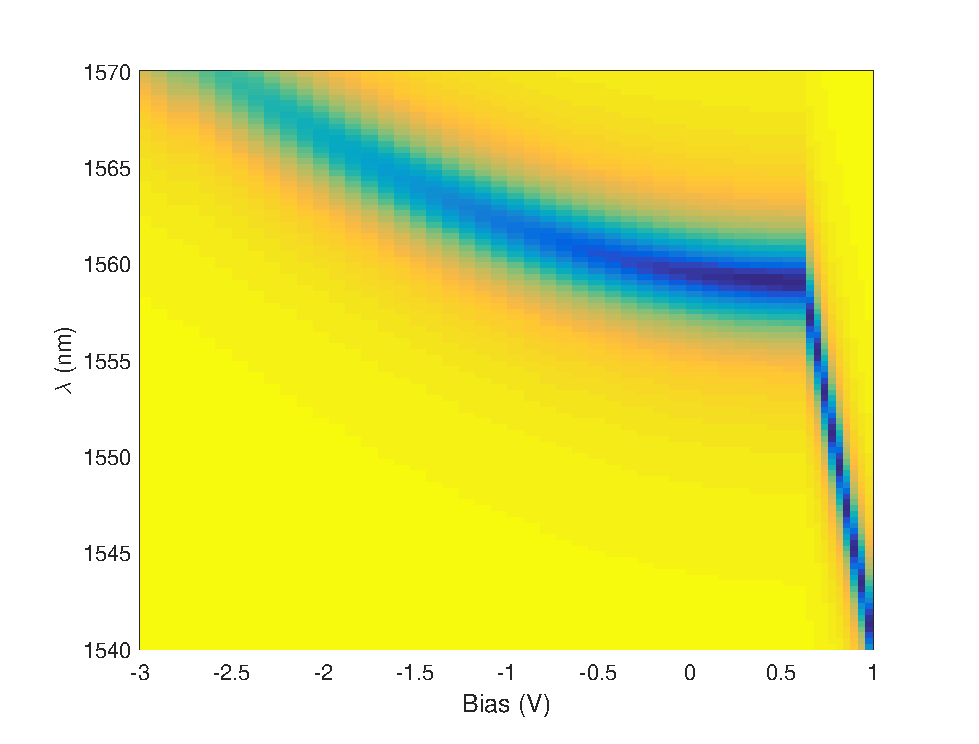
\includegraphics[width=14cm]{./Pictures/chapt4_bandfilling_sim.eps}
	\caption{80~$\mu m$长的电吸收光调制器在不同偏压下,计算得到的激子吸收谱。当偏压大于0.6~V时,激子吸收峰的漂移是基于能带填充效应,并且激子吸收峰强度保持20~dB以上。而小于0.6~V时,激子吸收峰的漂移是基于QCSE效应,激子吸收峰强度随着反偏电压的增加而减弱}
	\label{chapt4_bandfilling_sim}
\end{figure}

\section{混合集成调制器的制作}
硅基混合集成电吸收光调制器的制作,主要分成三个部分,第一个部分是硅波导的制作;第二个部分是键合工艺,在此我们采用基于DVS-BCB的粘贴键合工艺;第三部分是III-V波导和电极制作部分。下面我们就详细介绍各个步骤的流程。
\subsection{制作硅波导}\label{fab_siwg}
目前,SOI上的硅波导主要通过电子束光刻或者投影式光刻定义。电子束光刻是实验室中主要采用的方法,适合小批量,短周期的制作要求。而投影式光刻,由于设备昂贵则需要委托半导体公司流片。适合大批量,加工周期也一般比较长。这两种方式制作硅波导我们都尝试过。我们首先介绍利用电子束定义,加工硅波导。在此我们采用的是负胶ma-N~2403,其工艺步骤如下所示:
\begin{enumerate}[(1)]
	\item 匀保护胶。在大的SOI表面低速匀上保护的光刻胶,比如AZ~5214E,转速为2000~rpm,持续时间30~s。这用于保护片子,防止在后面解离步骤时,产生的碎末吸附在SOI表面。
	\item 解离SOI。用解离刀沿着晶向,划片子边沿,缺口长度尽可能小,大概3~mm左右即可,划的深度尽可能大。最后用解离钳解离片子。解离后的碎末用气枪吹干净。
	\item 清洗SOI。由于表面有一层光刻胶,因此用丙酮,异丙醇即可把表面光刻胶去除干净。为了将片子上的有机物彻底去除干净,可以将片子放到刚配好的H\SB{2}SO\SB{4} : H\SB{2}O\SB{2} = 1 : 1 的溶液中清洗,等待片子表面的气泡减少或者没有。
	\item 片子表面处理。为了提高SOI片子对ma-N~2403的粘附性,将片子放置到BOE中5s,然后用去离子水冲洗,氮气吹干。再放到120~$^{\circ}$C热盘上15~min去除水汽。
	\item 匀ma-N~2403胶。转速分别为 前转:1500~rpm, 3~s;后转:4000~rpm,30~s。分前转和后转是为了使光刻胶匀的更加均匀。
	\item 前烘光刻胶。将匀好的片子,放在90~$^{\circ}$C热盘90~s,这是为了蒸发光刻胶中的溶剂。
	\item 电子束曝光。 需要根据图形尺寸大小选择合适的曝光计量,电子枪运动的方式和图形划分的方式。我们写1.5~$\mu m$宽直波导的参数是,电子枪是30~KV, 20~$\mu m$,具体其他的参数需要时时调整。
	\item 显影。ma-N~2403 对应的显影液是Ma-D~525。在室温下,显影2 min 30 s,然后去离子水冲洗1~min,最后用氮气吹干,就可以得到图形。显好后片子截面示意图如图\ref{chapt4_3D_etch_siwg}(a)所示。
	\item 后烘回流。将片子放置在110~$^{\circ}$C的热盘上30~min,用于减小侧壁粗糙度,提高胶的耐刻蚀性。
	\item 刻蚀硅。将片子放在表面有很厚的SiO\SB{2}的Si托片上,送入ICP中刻蚀, 刻蚀结束后的波导截面示意图如图\ref{chapt4_3D_etch_siwg}(b)所示。
	\item 去胶。利用强力去胶剂和氧等离子体的去胶机,将已经部分碳化的硅波导上的光刻胶去除。去完胶的波导的截面示意图如如图\ref{chapt4_3D_etch_siwg}(c)所示,图\ref{chapt4_3D_etch_siwg}(d)是波导的电镜图。
	\item 套刻。通常硅波导和光纤是通过光栅结构进行光的耦合。当光栅的刻蚀深度和波导的刻蚀深度不同时,需要套刻光栅。此时需要将负胶ma-N~2403换成正胶比如PMMA胶或者ZEP胶。然后根据这两种胶的特性,重复第4步至11步,将其中的参数调整到对应光刻胶和图形的最佳参数。
\end{enumerate}

接下来,我们介绍委托半导体公司流片的过程。我们委托流片的公司是Imec\cite{Imec}。首先根据对方提供的器件库或者每个图层对应的刻蚀深度和材料绘制我们的器件。绘制好图形后,利用对方推荐的绘图工具比如Cadence Virtuoso或者Klayout,设置各个图层的颜色和顺序,预测最终加工完成的器件的形貌。在提交给对方工厂之前,我们还需要检查自己的图形是否符合对方工艺线流线,这就需要设计规则检查(Design Rule Check, DRC)。如果DRC检测通过,没有错误,那么就可以提交给对方公司流片。

利用电子束光刻加工的硅波导,由于工艺不稳定性,每个片子都会有些许不同,而且最后片子表面不平整,硅波导是突出的,但是加工周期可以自己可控。委托半导体公司流片,虽然工艺稳定些,但是他们是将一个小结构(Die)拼凑成一个大晶片(Wafer)进行加工。因此在大晶片不同位置上的小结构,尺寸也会有些许变化的。不过,半导体公司流片,由于对方工艺成熟,大型设备多,会将片子表面用SiO\SB{2}进行平坦化,这有益于后面的键合过程。

\begin{figure}[htb]
	\centering
	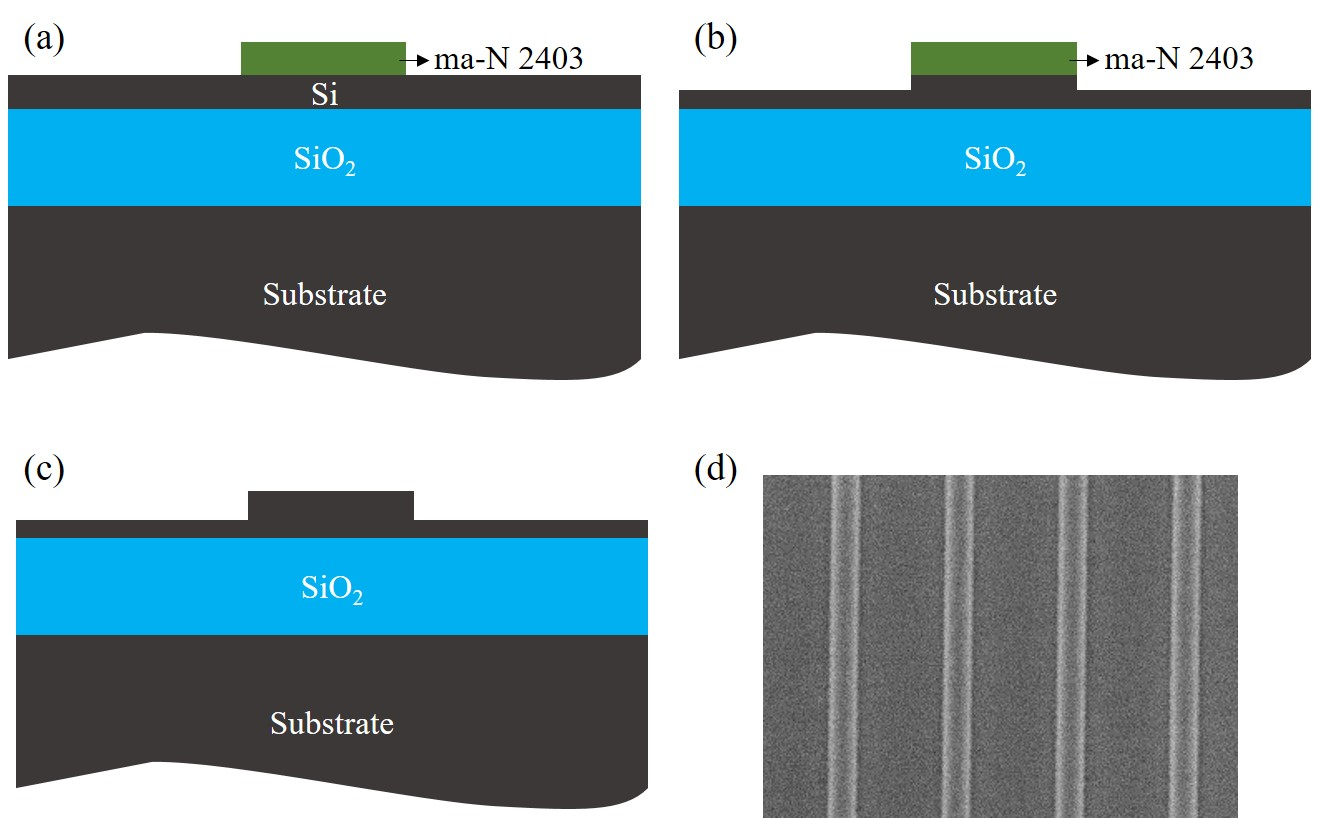
\includegraphics[width=14cm]{./Pictures/chapt4_3D_etch_siwg.jpg}
	\caption{(a)光刻胶定义图形;(b)通过干法刻蚀将图形转移到硅上;(c)去除光刻胶后,形成的硅波导;(d)实际硅波导的电镜图}
	\label{chapt4_3D_etch_siwg}
\end{figure}
\subsection{基于DVS-BCB的粘贴键合的工艺}
之所以使用基于DVS-BCB的粘贴键合工艺,是因为粘贴键合对片子表面的粗糙度要求低。即使是波导突出的SOI表面,粘贴键合依旧能完美地将III-V和SOI键合起来。粘贴键合主要分为11步,具体步骤如下:
\begin{enumerate}[(1)]
	\item 清洗硅片表面的有机物。用丙酮,异丙醇清洗,然后用去离子冲洗,氮气吹干。
	\item 清洗硅表面的颗粒。用标准的SC-1溶液(在75~$^{\circ}$C的NH\SB{3} : H\SB{2}O\SB{2} : H\SB{2}O = 1 : 1 : 5)清洗硅片15~min。再用去离子冲洗1~min,氮气枪吹干。
	\item 烘干硅表面。将硅片放置到120~$^{\circ}$C的热盘上3~min。
	\item 旋涂BCB。我们采用稀释过的DVS-BCB(Cyclotene\SP{®} 3022-35)\cite{dvsbcb35}使键合层的厚度小于50~nm\cite{keyvaninia2013ultra}。DVS-BCB : Mesitylene = 1:6的溶液,然后用转速3000~rpm, 时间40s。如果采用未被SiO\SB{2}平坦化后的硅片,则采用DVS-BCB : Mesitylene = 1 : 4的溶液,转速3000 rpm,40s。具体里的稀释比需要根据片子表面的高度差而定。
	\item 前烘BCB。将片子放置到150~$^{\circ}$C的热盘上5~min,然后自然冷却到70~$^{\circ}$C。使DVS-BCB中的溶剂和Mesitylene挥发。如果是未被SiO\SB{2}平坦化后的硅片,则需要先将片子放置到180~$^{\circ}$C的真空箱,或者氮气箱中,回流1~h,让片子表面的BCB变的更加平坦,最后也缓慢冷却到70~$^{\circ}$C。取出片子保存。此时硅片截面的示意图如图\ref{chapt4_bonding_diagram1}(a)所示。
	\begin{figure}[htb]
		\centering
		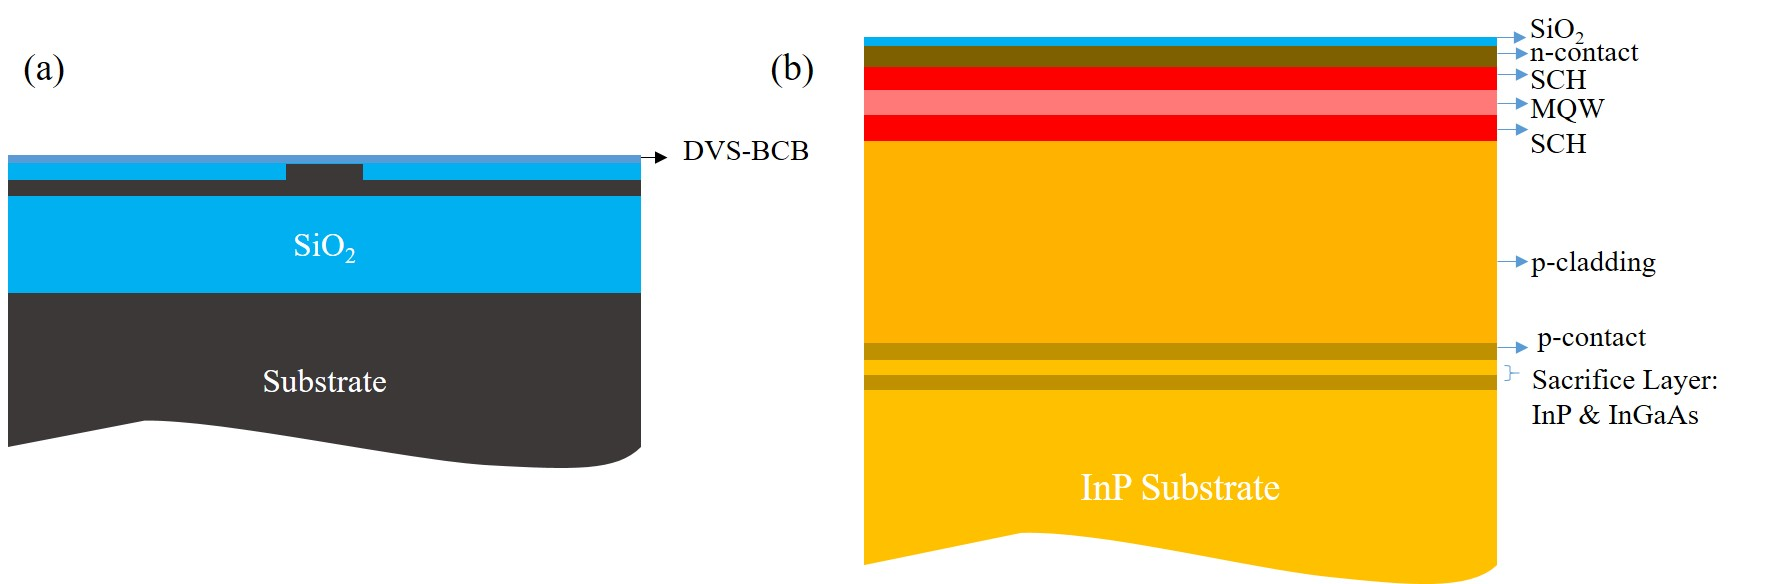
\includegraphics[width=14cm]{./Pictures/chapt4_bonding_diagram1.jpg}
		\caption{(a)匀上DVS-BCB的平坦化过的硅片截面示意图;(b)沉积SiO\SB{2}的III-V片子的截面示意图}
		\label{chapt4_bonding_diagram1}
	\end{figure}
	\item 解离III-V片子。将III-V相对比较大的片子,匀上光刻胶。再解离成合适大小的片子,解离时候注意晶向。波导需要沿着[0~1~-1]晶向的方向,这是因为用湿法腐蚀工艺的话,此时波导才会形成倒梯形。如果采用相垂直的方向,波导会形成正梯形。
	\item 清洗III-V片子。用丙酮和异丙醇,去除表面的光刻胶,然后吹干。在设计III-V的外延片时,我们一般还设计了两层200~nm厚的牺牲层InP/InGaAs。我们首先去除200~nm厚的InP牺牲层,通过将III-V片子放置到纯HCl中10s,然后用去离子水冲洗1~min,氮气吹干。然后我们再去除200~nm厚的InGaAs牺牲层,通过将III-V片子放置到H\SB{2}SO\SB{4} : H\SB{2}O\SB{2} : H\SB{2}O = 1 : 1 : 18的溶液中,腐蚀1~min,接下来用去离子水冲洗,氮气吹干。以上操作的溶液都是在20~$^{\circ}$C下进行。此时III-V表面露出干净的n-contact层。
	\item 沉积SiO\SB{2}。将III-V片子,放置到到120~$^{\circ}$C的热板上3~min,去除水汽。然后放置到PECVD中,沉积大概10~nm至20~nm的SiO\SB{2}。沉积SiO\SB{2}增加了III-V片子对DVS-BCB的粘附性。并且防止在湿法去除InP衬底时,HCl渗入BCB中,腐蚀n-contact层,导致键合的III-V片脱落。此时III-V片子的截面示意图如图\ref{chapt4_bonding_diagram1}(b)所示。
	\begin{figure}[htb]
		\centering
		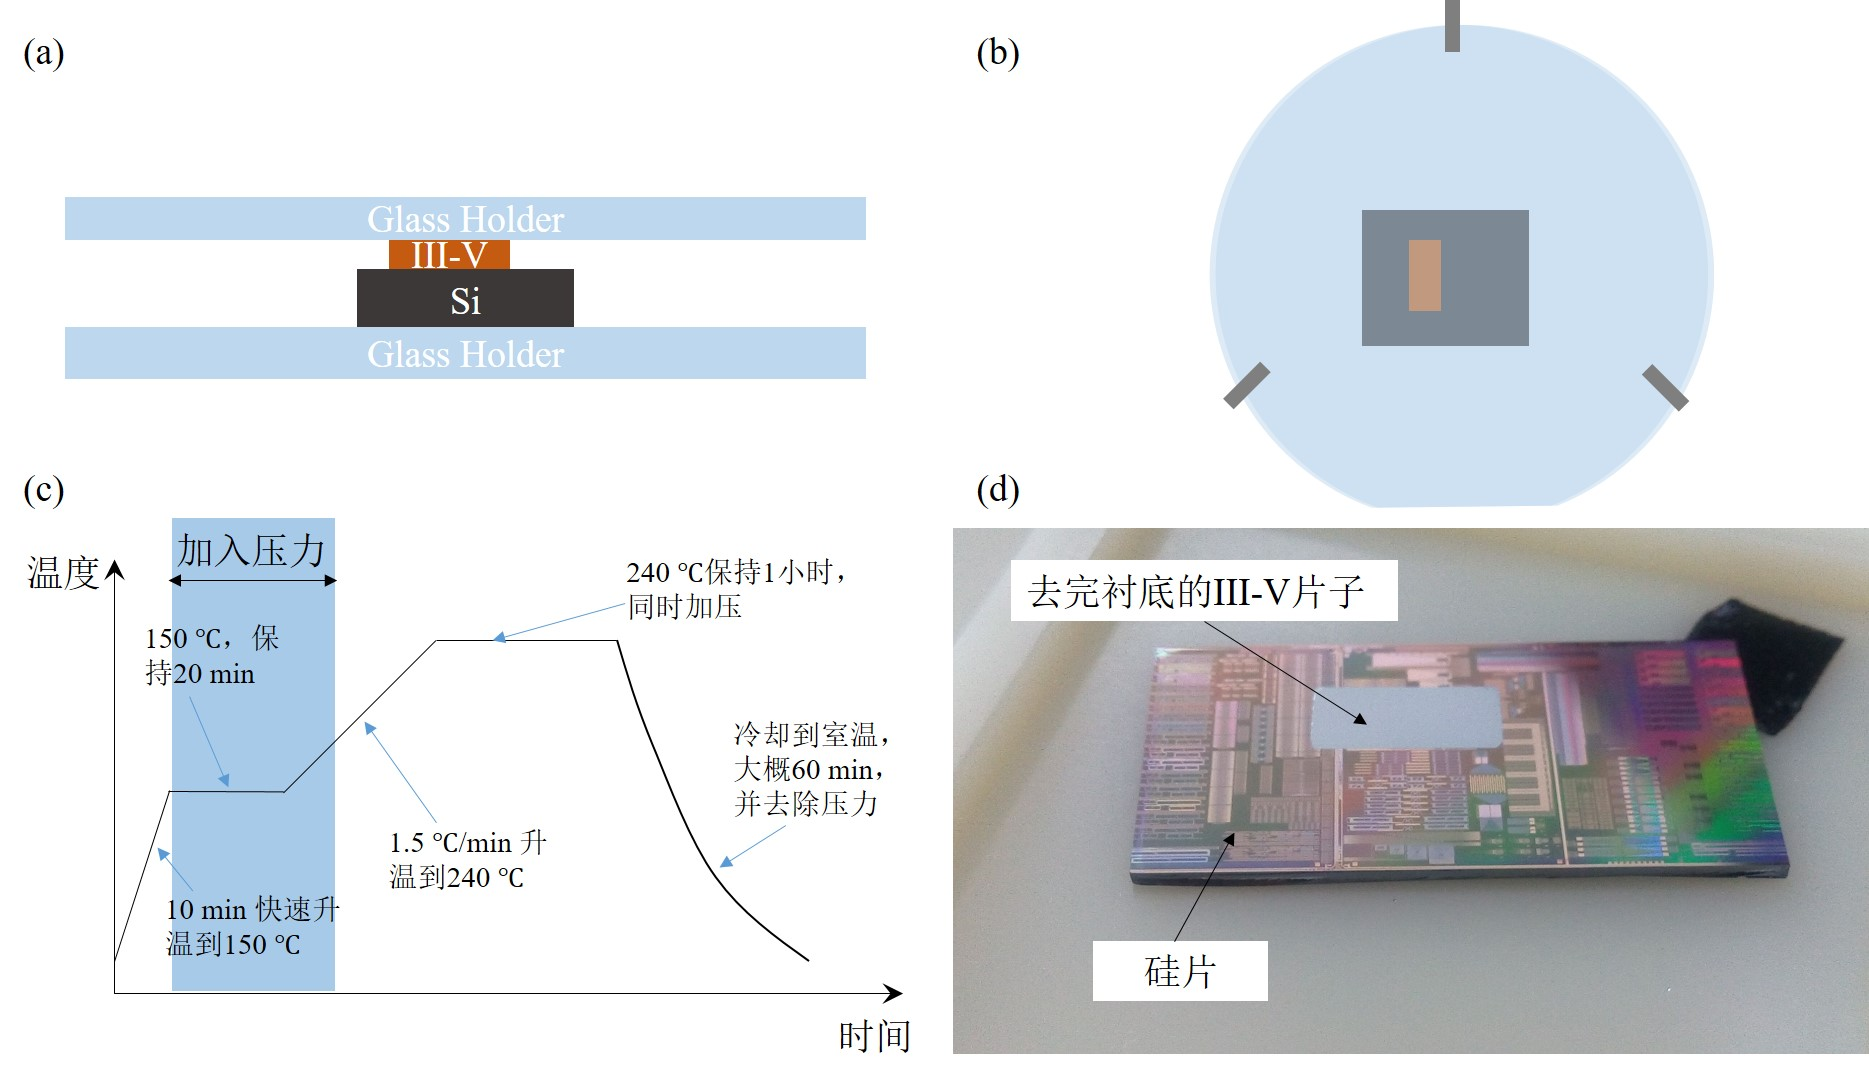
\includegraphics[width=14cm]{./Pictures/chapt4_bonding_diagram2.jpg}
		\caption{(a,b)分别展示了夹在石英玻璃间垒好的硅片和III-V片子的侧视和俯视示意图;(c)玻璃化DVS-BCB过程中的温度,以及施加压力的时刻;(d)实际去除完衬底,键合好的硅基混合集成III-V片子。}
		\label{chapt4_bonding_diagram2}
	\end{figure}
	\item 倒扣III-V片子到硅片上。在室温下,将III-V片子倒扣在硅片上。倒扣III-V片子,可以用弯曲的镊子夹住III-V片子边缘实现倒扣,也用真空洗笔吸附III-V片子背面将片子倒扣。倒扣III-V片子到硅片上后,可能III-V片子不再所想要的位置,此时,需要用薄镊子,小心将III-V片子推动到所需硅片上的位置。以上操作也可以用商用的倒装键合(Flip Chip)机器实现。
	\item 机器键合。我们使用商用的键合机器S{\"u}ss Microtec ELAN CB6L。由于这个商用键合机器是用于键合4英寸的片子,而我们的硅片也就5~cm$\times$5~cm以内。因此,我们需要将垒好的硅片和III-V片子,夹在4英寸的石英载玻片之间,如图\ref{chapt4_bonding_diagram2}(a,b)所示。随后,我们将其放入键合机的腔体内,进行在真空环境中的键合。我们可以控制腔体的温度,如图\ref{chapt4_bonding_diagram2}(c)所示,将DVS-BCB玻璃化。当温度上升到150~$^{\circ}$C时,DVS-BCB还是保持流动状态,因此我们对两个石英片加入上下的压力,通过压力,能经一步减小III-V和硅片之间的DVS-BCB的厚度,同时将III-V片子和硅片表面间的空隙被DVS-BCB填慢。当温度大于180~$^{\circ}$C时,我们释放压力,以防玻璃化后的DVS-BCB受到额外的应力。
	\item 去除InP衬底。我们将键合好的片子放置到温度为40~$^{\circ}$C的HCl : H\SB{2}O = 4 : 1的溶液中。当没有气泡产生时,表明衬底已经去除干净。如果III-V片子边缘依旧有残留的衬底,尤其沿着[0~1~1]方向使。可以在匀上光刻胶后,用小刀刮掉,再用丙酮,异丙醇,去离子冲洗干净。键合后的III-V片子如图\ref{chapt4_bonding_diagram2}(d)所示。
\end{enumerate}	

虽然基于DVS-BCB的粘贴键合工艺对片子的粗糙度要求低,但是硅表面和III-V表面最好保持干净。因为在机器键合加压力时,脏颗粒,可能将局部的III-V顶破,甚至是局部脱落,或者引入气泡,如图\ref{chapt4_bonding_error}所示。这些现象,只有在去除完InP衬底后,才能看到。在键合过程中,除了保持硅片和III-V表面的干净,其中最终要的步骤,就是在III-V片子上表面沉积很薄的SiO\SB{2},防止在去除InP衬底时,III-V片子脱落。
\begin{figure}[htb]
	\centering
	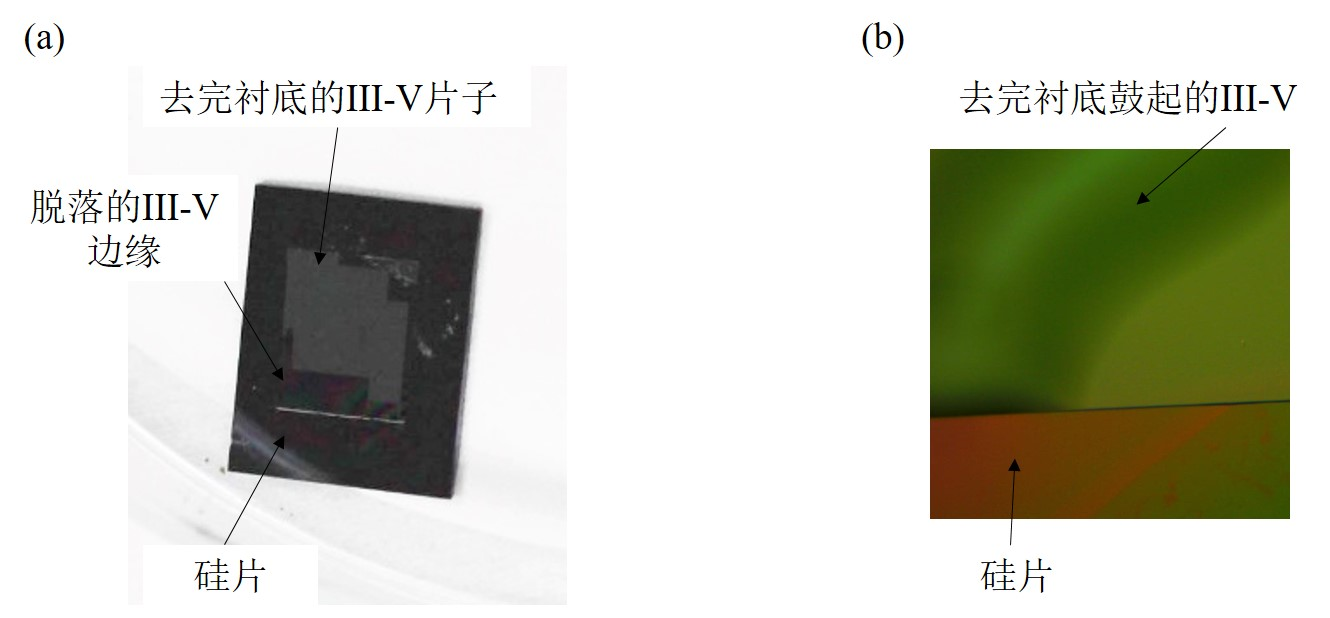
\includegraphics[width=14cm]{./Pictures/chapt4_bonding_error.jpg}
	\caption{展示了由于键合前III-V表面没有长SiO\SB{2}导致键合失败的例子。(a) III-V片子边缘脱落;(b) III-V片子局部出现气泡鼓起。}
	\label{chapt4_bonding_error}
\end{figure}
\subsection{制作III-V波导}
我们根据现有的混合集成III-V波导的制作流程\cite{roelkens2015iii},简化了工艺步骤,实现了全湿法制作混合集成III-V波导的新工艺流程。新工艺的详细步骤见图\ref{chapt4_III_V_wg_process}。下面将详细介绍每一步的工艺流程。下面的湿法步骤都是在溶液温度为20~$^{\circ}$C时进行的。
\begin{figure}[!h]
	\centering
	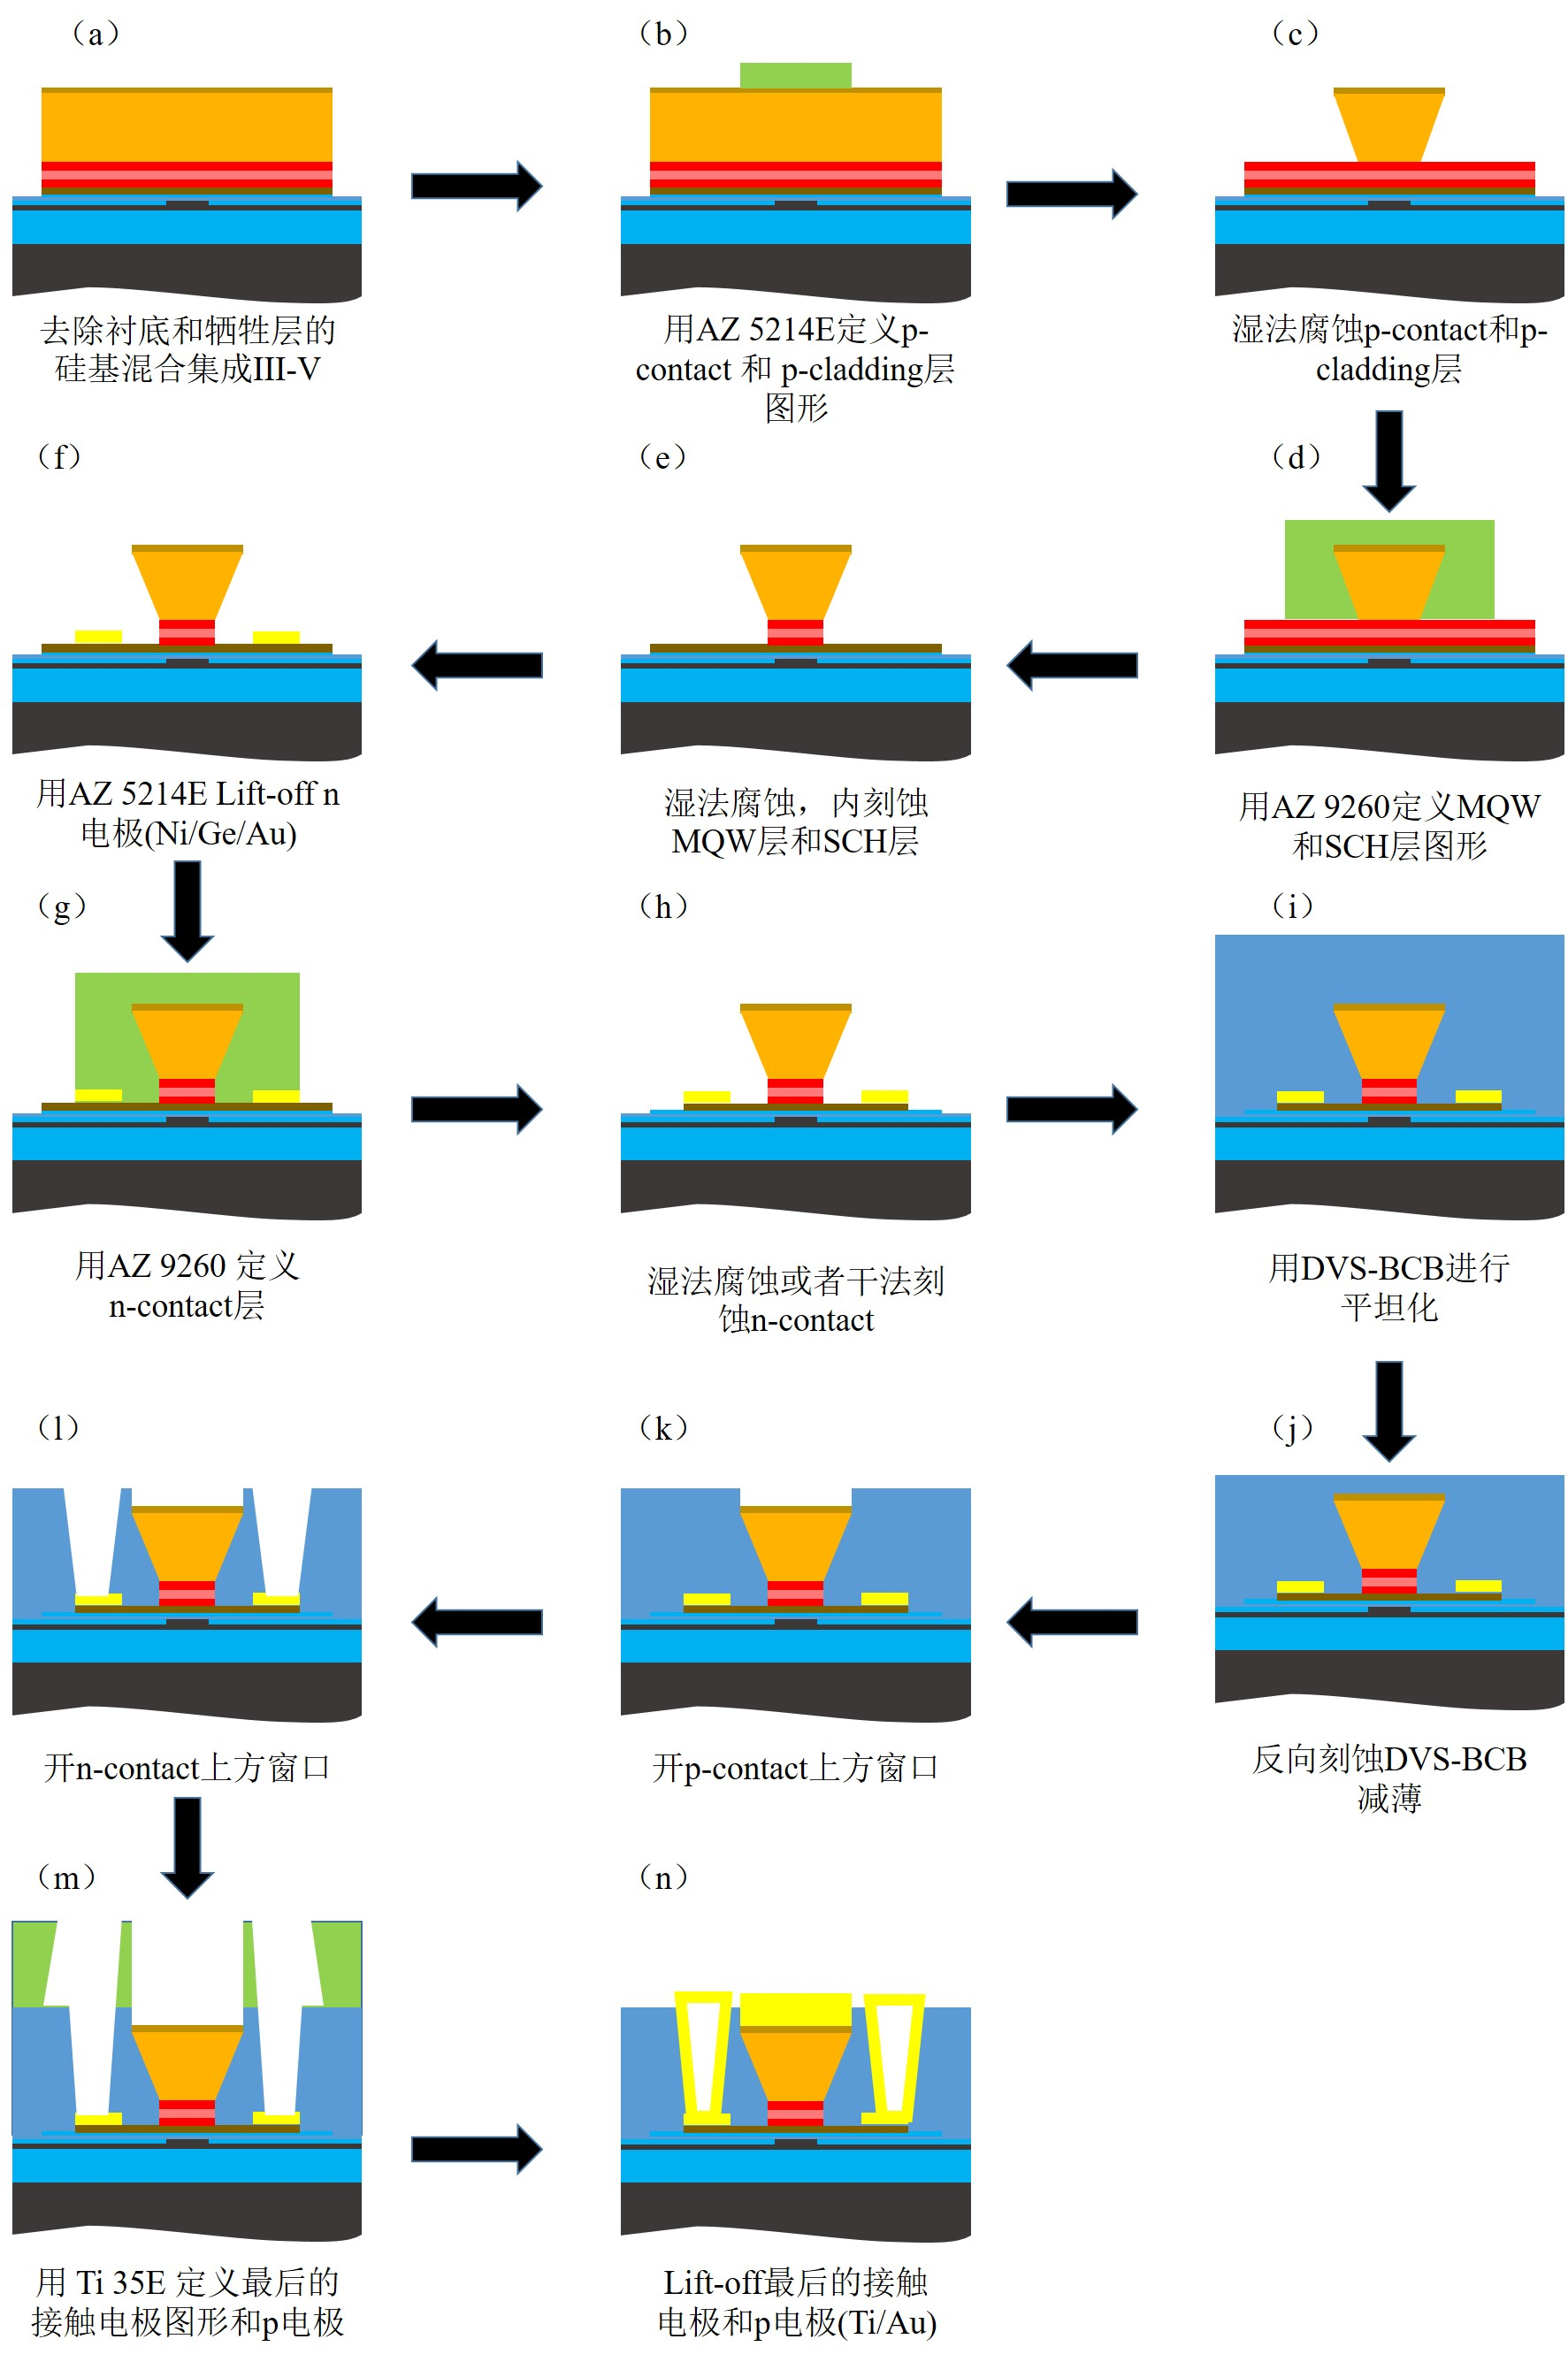
\includegraphics[width=14cm]{./Pictures/chapt4_III_V_wg_process.jpg}
	\caption{制作硅基混合集成III-V波导的工艺流程示意图,展示了波导截面在不同步骤下的形貌示意图。}
	\label{chapt4_III_V_wg_process}
\end{figure}

第一步,去牺牲层。将p-contact层上面的两层牺牲层湿法去除。去除第一层牺牲层InGaAs用H\SB{2}SO\SB{4} : H\SB{2}O\SB{2} : H\SB{2}O = 1 : 1 : 18的溶液,腐蚀1~min。去除第二层牺牲层用纯HCl,腐蚀10 s。去除结束后的混合集成III-V片子的截面图,如图\ref{chapt4_III_V_wg_process}(a)所示。

第二步,以硅片上的标记为基准,套刻第一层图像。我们先对p-contact表面进行处理,提高其对光刻胶的粘附性。我们将片子放置到120~$^{\circ}$C的热盘上,烘烤3~min,再匀增粘剂Ti Primer,转速 3000~rpm, 40~s。随后,烘烤120 ~$^{\circ}$C, 3~min。此时片子表面处理完,开始匀光刻胶AZ~5214E定义图型。AZ~5214E定义图形最窄的线条宽度为$1~\mu m$。匀AZ~5214E胶的转速为 3000~rpm,时间为 40~s。接下来,将片子放置到100~$^{\circ}$C的热盘上,烘烤 3~min。接下来,用接触式光刻机进行曝光。最后进行显影,等到片子表面的彩色条纹全部褪去。 此时,混合集成III-V片子的截面图,如图\ref{chapt4_III_V_wg_process}(b)所示。

第三步,湿法腐蚀p-contact层。我们以光刻胶为mask,湿法腐蚀InGaAs,溶液是H\SB{3}PO\SB{4} : H\SB{2}O\SB{2} : H\SB{2}O = 1 : 1 : 20。腐蚀过程中,准确控制腐蚀深度。以防湿法腐蚀过头,导致InGaAs宽度变窄。

第四步,去除光刻胶。我们用丙酮,异丙醇清洗光刻胶AZ~5214E。为了保证光刻胶去除干净,我们再用氧离子清洗机,清洗。

第五步,湿法腐蚀p-cladding层。我们以p-contact为掩膜,用HCl : H\SB{2}O = 1 : 1的溶液腐蚀p-InP层。腐蚀结束后,p-InP层会形成倒梯形。左右上顶角的角度为70°左右。此时,混合集成III-V片子的截面图,如图\ref{chapt4_III_V_wg_process}(c)所示。在腐蚀结束后,第一层图形中锥形结构上的InGaAs会坠下来,落在SCH层上,如图\ref{chapt4_III_V_suspeneded_InGaAs}所示。由于InGaAs对$1.55~\mu m$的光波会有强烈的吸收,因此需要将悬挂部分的InGaAs去除掉。
\begin{figure}[!h]
	\centering
	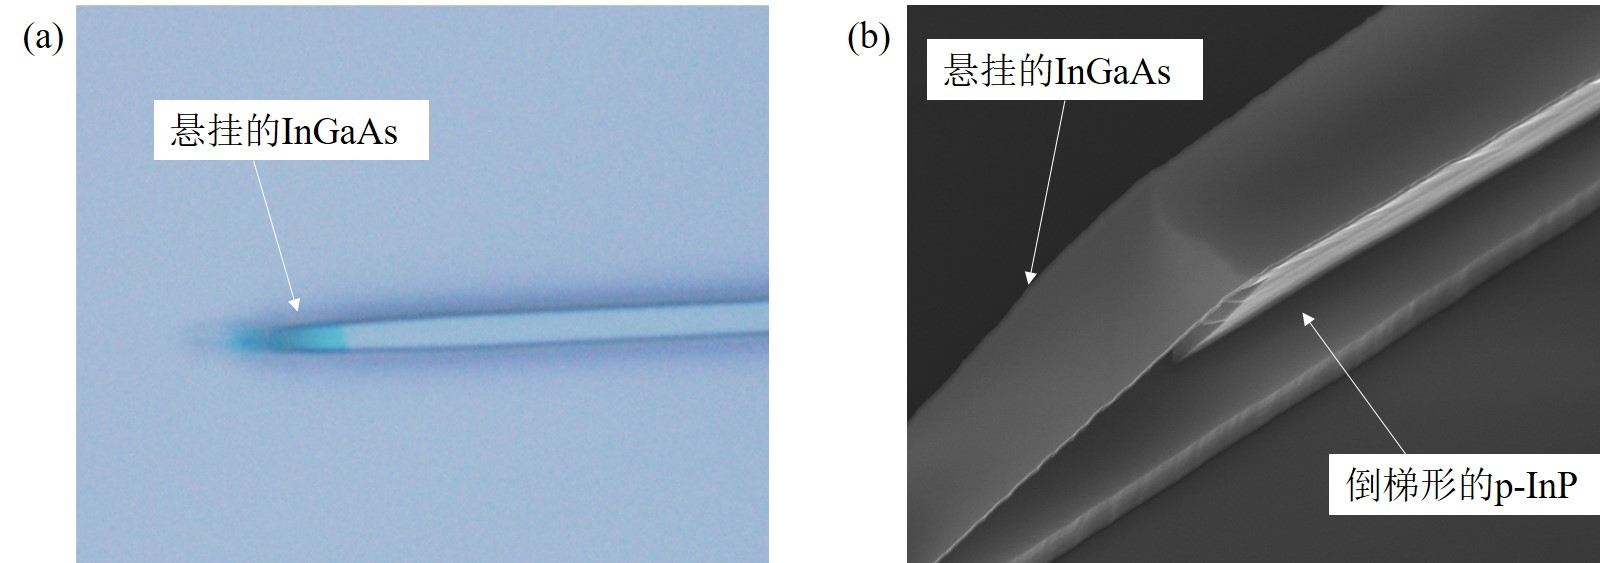
\includegraphics[width=14cm]{./Pictures/chapt4_III_V_suspeneded_InGaAs.jpg}
	\caption{悬挂的InGaAs层。(a)显微镜图;(b)电镜图}
	\label{chapt4_III_V_suspeneded_InGaAs}
\end{figure}

第六步,去除悬挂的InGaAs。去除悬挂可以采用一次光刻套刻,只露出悬挂部分的InGaAs,再湿法腐蚀将其去除。在此我们首次采用更为简单的超声法去除悬挂。由于超声会在液体中产生震动,对于悬挂的InGaAs薄膜很容易在震动中断裂。因此,可以用于去除悬挂的InGaAs。由于超声机产生的震动并不是均匀的,因此会导致部分悬挂去除,而其他地方的悬挂依旧保留的情况,甚至波导被震裂,如图\ref{chapt4_III_V_remove_InGaAs}所示。不过,通过合理控制超声功率,可以只将悬挂处的InGaAs去除。
\begin{figure}[!h]
	\centering
	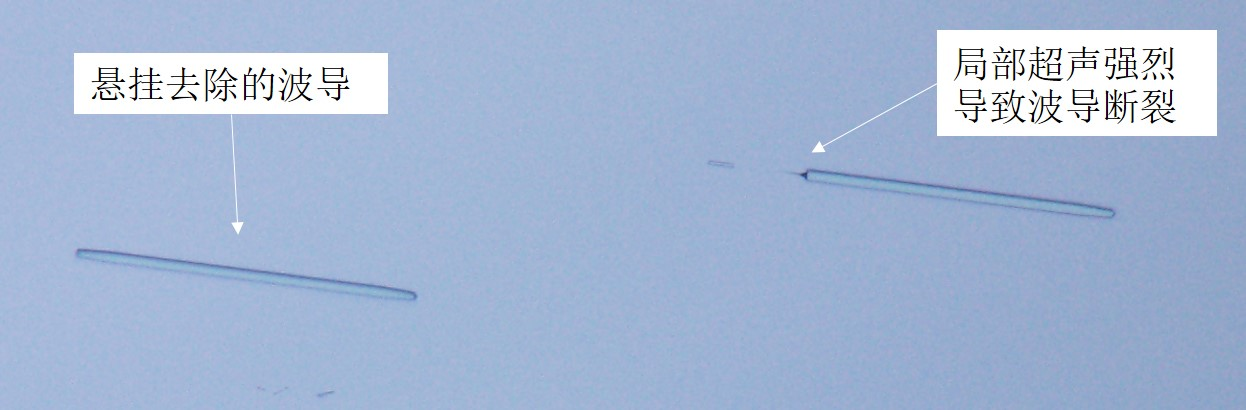
\includegraphics[width=14cm]{./Pictures/chapt4_III_V_remove_InGaAs.jpg}
	\caption{悬挂的InGaAs层。(a)显微镜图;(b)电镜图}
	\label{chapt4_III_V_remove_InGaAs}
\end{figure}

第七步,套刻第二层MQW层和SCH层上的图形。步骤也是与第二步相同,用Ti Primer对片子表面进行处理。然后,我们用更加厚的光刻胶AZ~9260 (大概$5~\mu m$),定义图形。AZ~9260所需的转速是 6000~rpm,时间40~s。接下来,我们进行仔细的套刻,套刻偏差需要小于200~nm。然后进行曝光显影。此时,混合集成III-V片子的截面图,如图\ref{chapt4_III_V_wg_process}(d)所示。

第八步,湿法腐蚀量子阱。我们采用柠檬酸(Citric) : H\SB{2}O\SB{2} = 1 : 1的溶液进行腐蚀。由于我们光刻胶定义的波导宽度大于实际宽度,因此我们需要内腐蚀(undercut),使波导的宽度变窄。在实验中,我们发现波导的斜率在腐蚀的过程中并不会改变。利用这个特点,我们可以在掩膜中将锥形的宽度展宽,长度延长。在内腐蚀后,波导宽度就会变窄,长度也会缩短。图\ref{chapt4_III_V_undercut_MQW}(a)展示了以SiO\SB{2}为掩膜时,内腐蚀过程中量子阱的宽度比掩膜的图形小。但是光刻胶为掩膜,我们无法观测到掩膜下面波导的宽度。因此我们采用如图\ref{chapt4_III_V_undercut_MQW}(b)中宽度不同的直波导,当内腐蚀程度大于直波导的宽度,直波导的胶飘落,以此可以来预测內腐蚀的程度。图\ref{chapt4_III_V_undercut_MQW}(c)展示了,腐蚀结束后的MQW层和SCH层的尖端。可看到,MQW层和SCH层也被腐蚀成了倒梯形。并且侧壁不是完美的光滑直线。因此这也会导致额外的损耗。做完这步后,混合集成III-V片子的截面图,如图\ref{chapt4_III_V_wg_process}(d)所示。
\begin{figure}[!h]
	\centering
	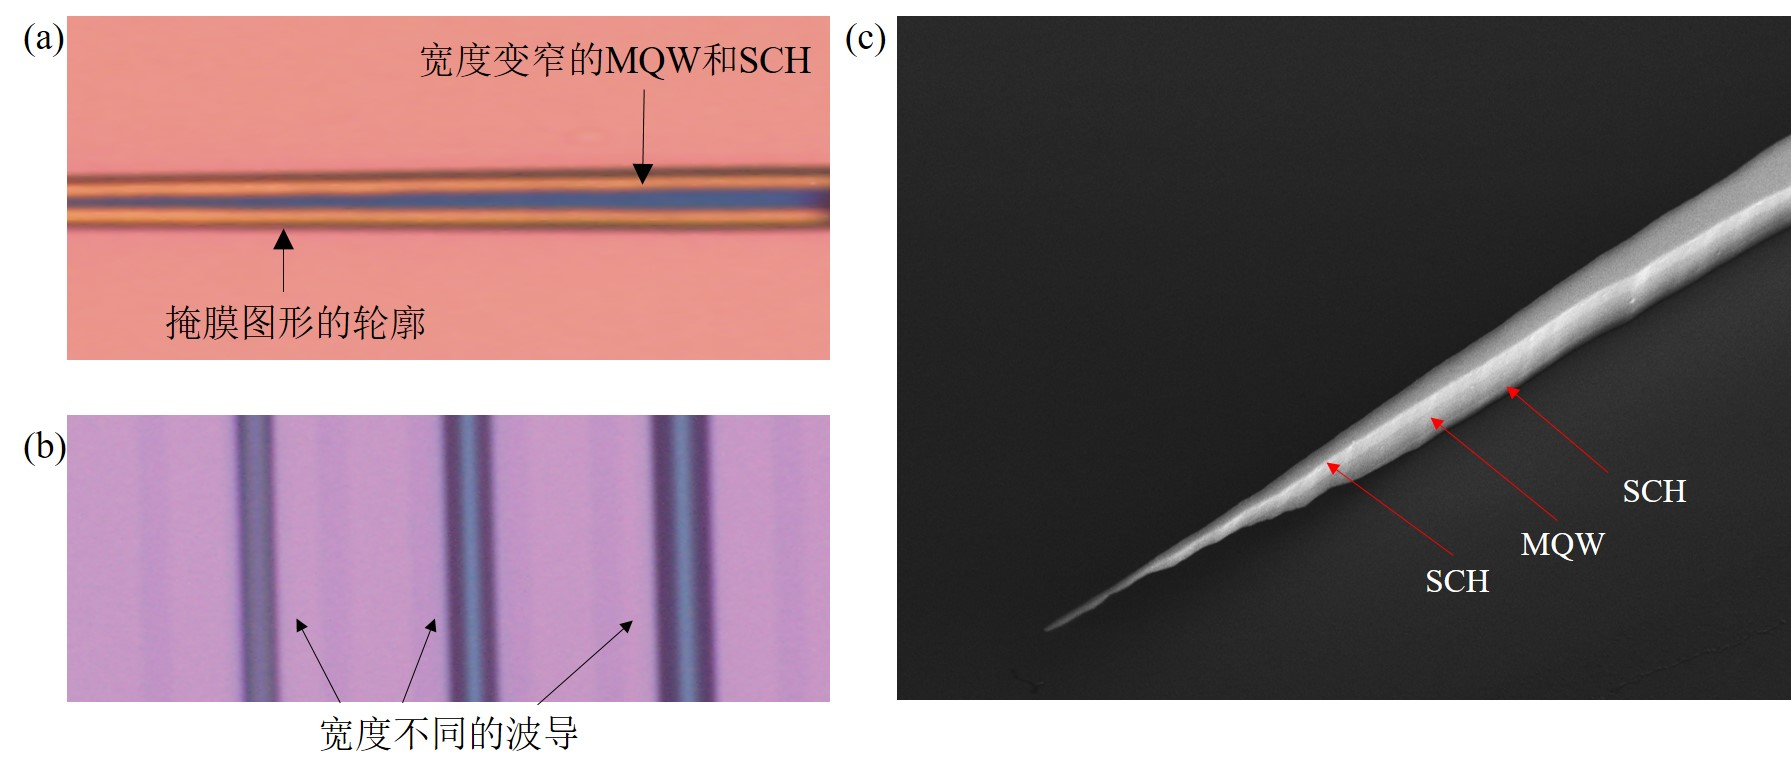
\includegraphics[width=14cm]{./Pictures/chapt4_III_V_undercut_MQW.jpg}
	\caption{悬挂的InGaAs层。(a)显微镜图;(b)电镜图}
	\label{chapt4_III_V_undercut_MQW}
\end{figure}

第九步,定义n金属电极的图形。我们采用正胶Ti~35E。Ti~35E可以做图像反转,显影后形成倒梯形结构,适合做金属的Lift-off。先用丙酮,异丙醇和去离子水将片子表面的光刻胶去除干净,用氮气枪吹干。然后放置到温度为120 ~$^{\circ}$C的热板上烘干。接下来,我们用3000~rpm,40~s的参数匀上Ti~35E。先在100 ~$^{\circ}$C下,前烘3~min,再套刻曝光,静置10~min。随后,进行放置到123 ~$^{\circ}$C的热盘上,烘2~min。然后,在无掩膜的情况下曝光185~s。最后,进行显影。此时,可以在显微镜下观察,由于倒梯形的关系,光刻胶的图形边缘会有两层轮廓。

第十步,溅射n金属,我们首先将显影结束的片子放置到反应等离子刻蚀机(Reactive Ion Etching,RIE)中,氧清洗30~s,确保Ti~35E孔内没有光刻胶残留。然后,用H\SB{2}SO\SB{4} : H\SB{2}O\SB{2} : H\SB{2}O = 1 : 1 : 50的溶液浸泡5~s。接下来,在溅射机中,溅射金属30~nm的Ni,20~nm的Ge,50~nm的金。最后,取出溅射好的片子,放置到丙酮中,剥离(Lift-off)金属。此时,混合集成III-V片子的截面图,如图\ref{chapt4_III_V_wg_process}(f)所示。

第十一步,定义n-contact图形。匀胶光刻和显影步骤与第七步相同。此时的波导结构如图\ref{chapt4_III_V_wg_process}(g)所示。

第十二步,刻蚀n-contact层图形。n-contact层的材料也是InP,因此,我们采用HCl : H\SB{2}O = 1 : 1的溶液进行腐蚀。不过,我们实验发现,重掺n型的InP,其侧向的腐蚀速率比掺p型的InP的侧向腐蚀速率快。另外,金属附近的InP侧向腐蚀几乎没有。如果,n-contact层也需要是锥形形状,可以采用干法刻蚀获得。此时,混合集成III-V片子的截面图,如图\ref{chapt4_III_V_wg_process}(h)所示。

第十三步,匀DVS-BCB进行平坦化。在匀DVS-BCB之前,我们需要去除III-V侧壁在空中产生的氧化层。我们将片放置在BOE : H\SB{2}O = 1 : 1 的溶液中浸泡1~min。由于我们III-V波导的台阶有3层,并且高度差也有$2 \mu m$以上,为了使DVS-BCB充分填充III-V波导,我们首先匀DVS-BCB35 (Cyclotene\SP{®} 3022-35)\cite{dvsbcb35} : Mesitylene = 1:4的溶液,转速1000~rpm, 40~s.然后匀纯的DVS-BCB46(Cyclotene\SP{®} 3022-46)\cite{dvsbcb46},转速3000~rpm, 40~s。接着将片子送入氮气箱,用图\ref{chapt4_bonding_diagram2}(c)的曲线,在不加压力的情况下玻璃化DVS-BCB。波导的截面示意图如图\ref{chapt4_III_V_wg_process}(i)所示。

第十四步,反向刻蚀DVS-BCB。我们使用ICP采用SF6 : O\SB{2} = 50 : 5的气体,刻蚀DVS-BCB。使BCB的上表面距离p-contact的上表面还剩下300~nm左右。波导的截面示意图如图\ref{chapt4_III_V_wg_process}(j)所示。

第十五步,在p-contact上开孔。我们首先按照第九步的Ti~35E工艺配方,定义p-contact孔的图形。然后,用第十四步的刻蚀DVS-BCB的配方,将p-contact上的DVS-BCB刻蚀干净。波导的截面示意图如图\ref{chapt4_III_V_wg_process}(k)所示。

第十六步,在n电极上开孔。与第十五步相同,以n电极的图形为掩膜,开孔。此时,波导截面的示意图如\ref{chapt4_III_V_wg_process}(l)所示。

第十七步,定义p电极和接触电极。这步与第九步的工艺步骤相同。结束后,波导的截面示意图如图\ref{chapt4_III_V_wg_process}(m)所示。

第十八步,溅射p电极和接触电极。我们首先将显影结束的片子放置到反应等离子刻蚀机(Reactive Ion Etching,RIE)中,氧清洗30~s,确保待溅射孔内的没有光刻胶残留。然后用H\SB{2}SO\SB{4} : H\SB{2}O\SB{2} : H\SB{2}O = 1 : 1 : 50的溶液浸泡5~s。接下来,在溅射机中,溅射金属40~nm的Ti,1~$\mu m$的金。最后,将溅射好的片子放置到丙酮中,剥离(Lift-off)金属。此时,混合集成III-V片子的截面图,如图\ref{chapt4_III_V_wg_process}(n)所示。最后制作成功的硅基混合集成III-V调制器的波导截面电镜图和调制器整体结构显微镜图如图\ref{chapt4_III_V_results}所示。
\begin{figure}[htb]
	\centering
	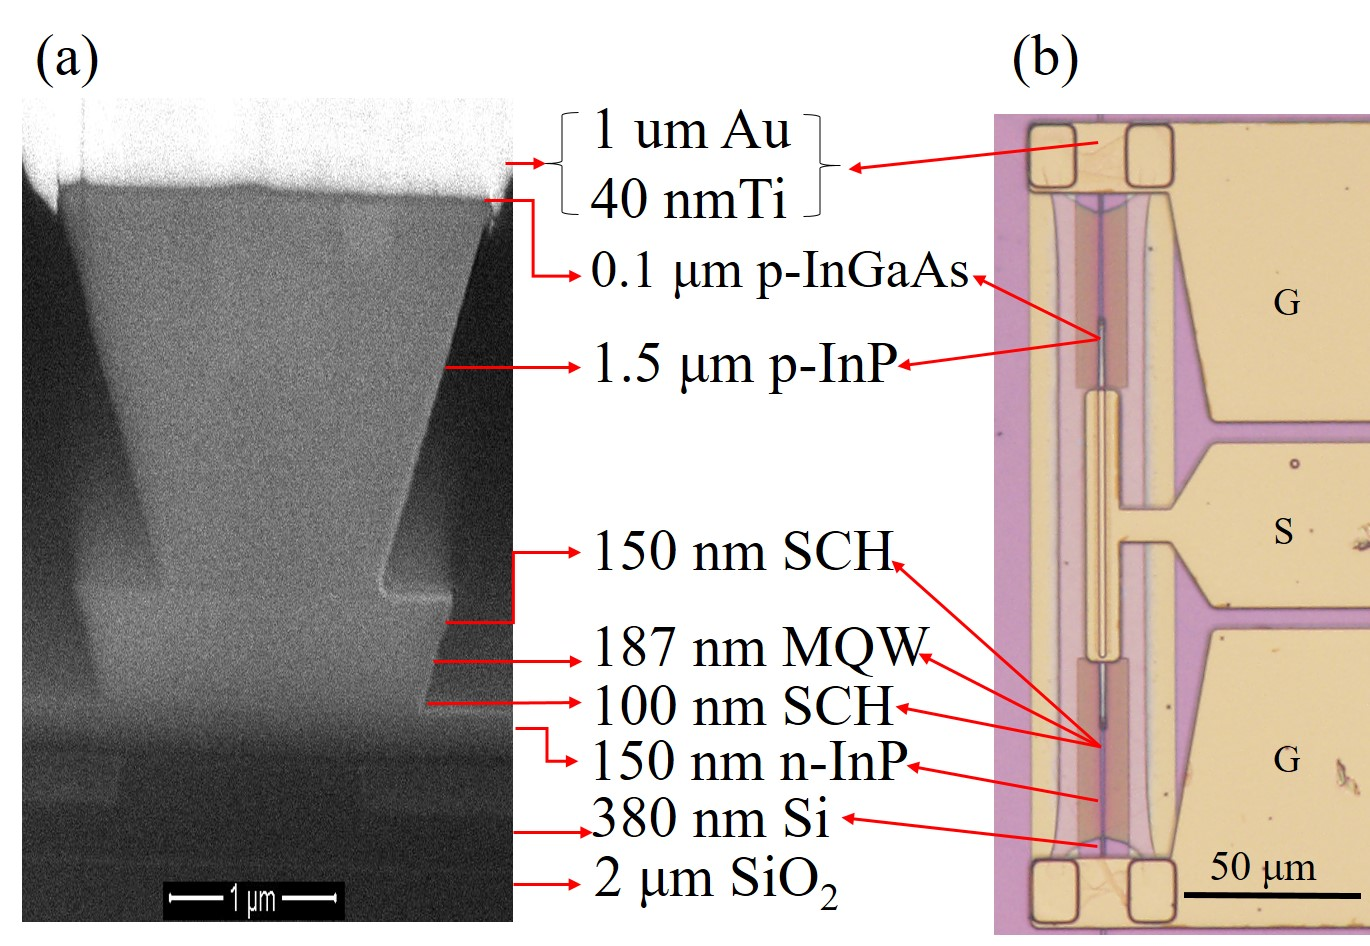
\includegraphics[width=12cm]{./Pictures/chapt4_III_V_results.jpg}
	\caption{硅基混合集成调制器(a)波导截面电镜图;(b)调制器整体结构显微镜图}
	\label{chapt4_III_V_results}
\end{figure}

虽然纯湿法制作III-V波导能够简化工艺步骤,但是有三个步骤有一定的风险。第一个是第六步去除悬挂的InGaAs。如果超声不均匀可能将波导损坏,或者部分InGaAs可能落在III-V波导上,如图\ref{chapt4_III_V_wrong_results}(1)所示,从而导致额外的损耗。第二个是MQW层和SCH层的套刻精度,套刻偏差大,将导致硅波导到III-V波导的耦合效率降低,如图\ref{chapt4_III_V_wrong_results}(2)。第三个是腐蚀MQW层和SCH层如果用不正确的腐蚀液比如使用H\SB{3}PO\SB{4},H\SB{2}O\SB{2},H\SB{2}O的混合液,就会导致锥形结构的侧壁粗糙度显著增加,如图\ref{chapt4_III_V_wrong_results}(3)所示。
\begin{figure}[htb]
	\centering
	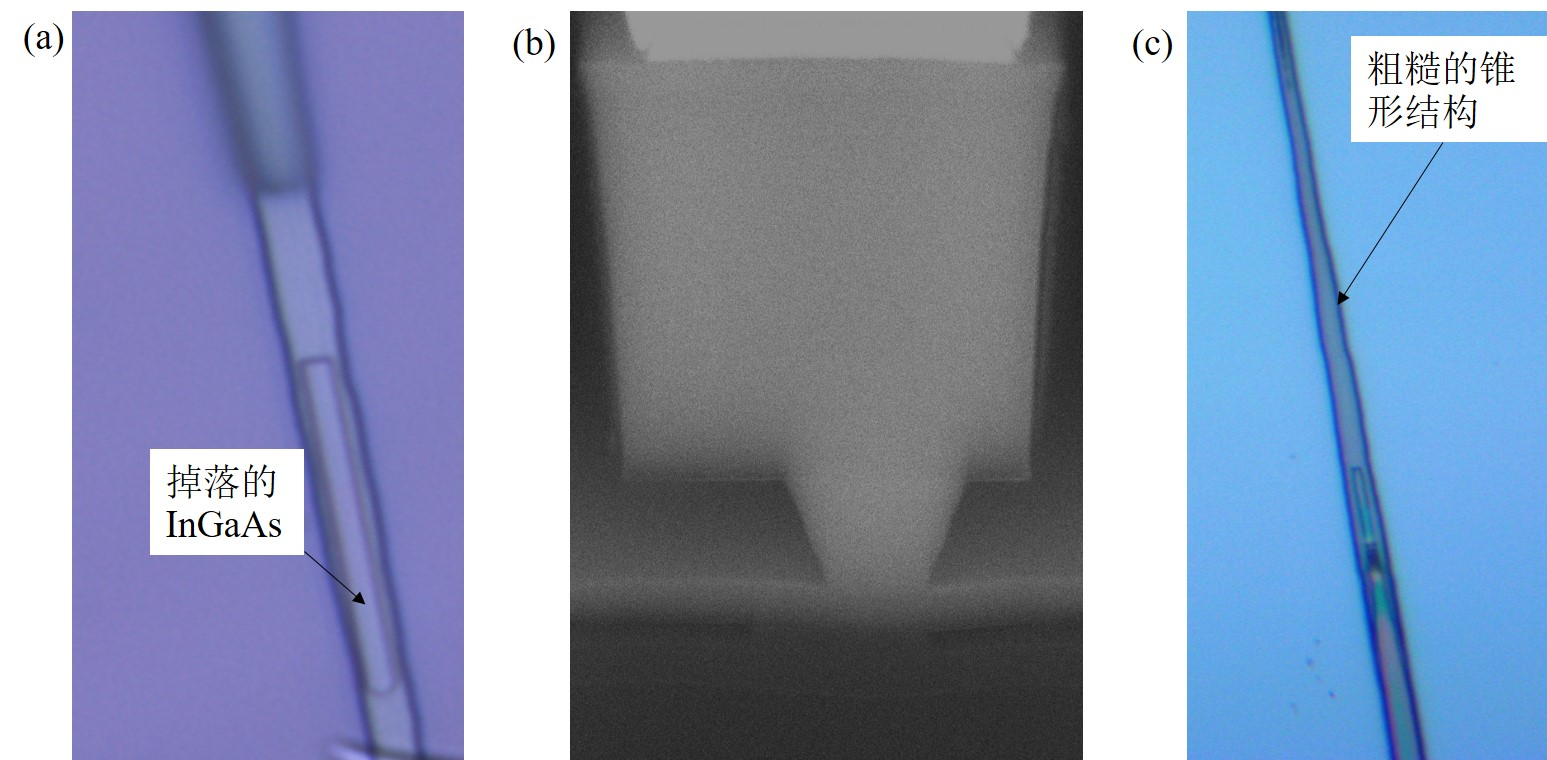
\includegraphics[width=14cm]{./Pictures/chapt4_III_V_wrong_results.jpg}
	\caption{(a)悬挂的InGaAs掉落到SCH上;(b)MQW层和SCH层的套刻误差;(c)MQW层和SCH层锥形结构粗糙的侧壁}
	\label{chapt4_III_V_wrong_results}
\end{figure}

\subsection{金属电极退火}
制作完硅基混合集成III-V电吸收光调制器后,就需要进行I-V测试。由于III-V材料,整体是一个pin结构,所以I-V曲线也是标准的二极管曲线。当接触电阻过大时,我们就需要对器件进行快速退火,改善金属与p-contact,n-contact间的接触。在此,我们采用的是电压快速退火法。通过加载一个比较高的电压,利用焦耳热直接对电极进行退火。这种方法的优点是,可以对单个器件进行操作,不需要快速退火炉,直接在测试过程中进行退火,单个器件的退火速度快,适合实验中使用。缺点是电流太大可能将器件烧坏,如果所有器件都需要退火,那么这种方法退火速度慢。

图\ref{chapt4_3D_resist}(a)中,退火前的曲线,是我们将电压从-1~V逐渐增高到2~V时获得的。可以看到,此时的正向导通电阻受到金属和半导体接触电阻的限制,有$3.5~ \Omega \cdot mm$。然后,我们将电压从-1~V提高到3~V,为了防止器件被烧坏,我们将电流最大值限制在50~mA,其I-V曲线见图\ref{chapt4_3D_resist}(b)。从中可以看到,当电压在2.3~V时,电流瞬间变大,表明电阻瞬间减小,从而说明退火成功,接触电阻减小了。随后,我们再次将电压从-1~V提高到2~V,可以看到接触电阻减小到了$2.3~ \Omega \cdot mm$。
\begin{figure}[htb]
	\centering
	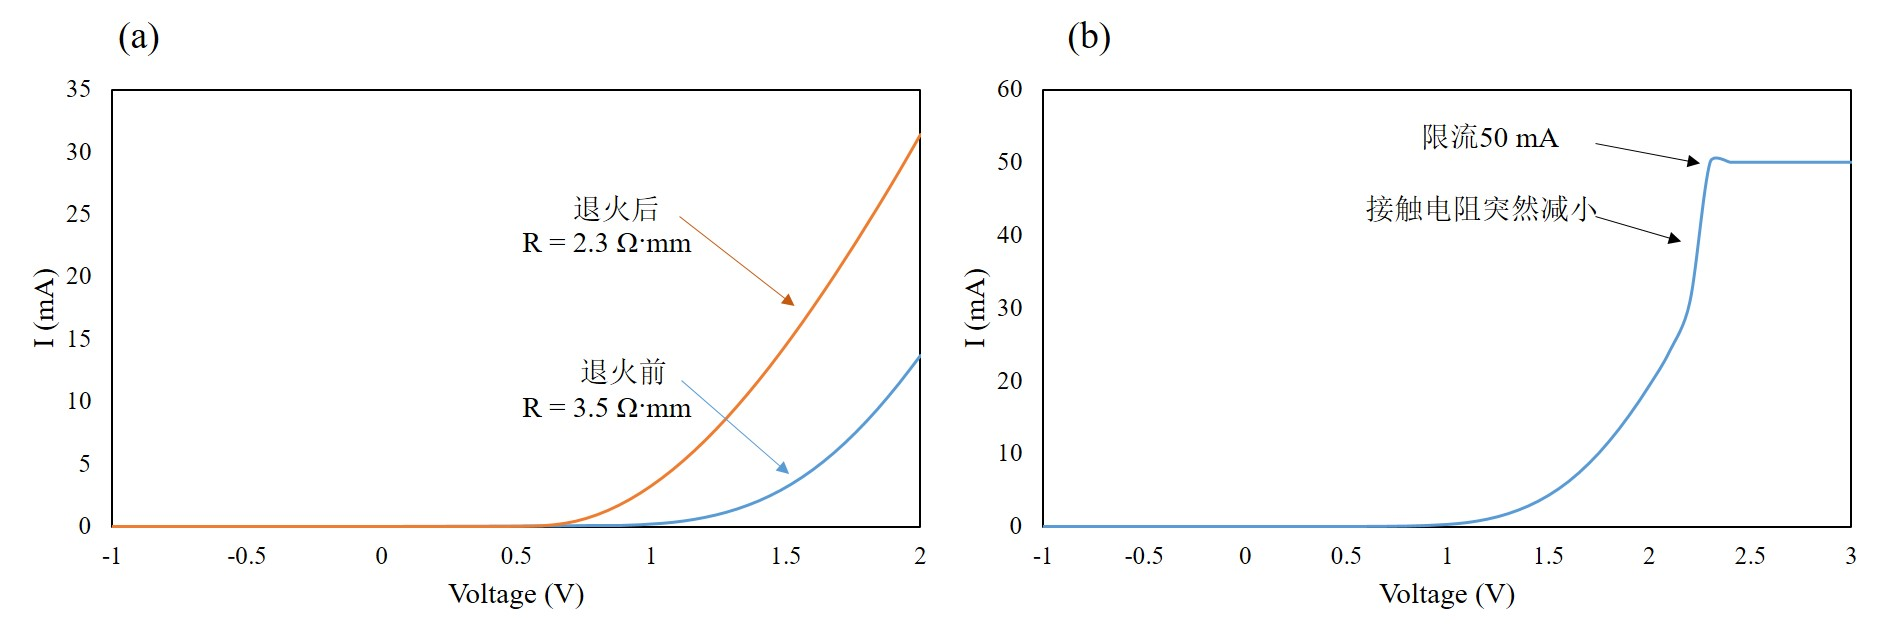
\includegraphics[width=15cm]{./Pictures/chapt4_3D_resist.jpg}
	\caption{(a)退火前和退火后调制器的I-V曲线;(b)利用电压快速退火法时,调制器的I-V曲线。在2.3~V出现电流突然增大,对应的电阻瞬间降低,从而说明退火成功,接触电阻减小}
	\label{chapt4_3D_resist}
\end{figure}
\section{硅基混合集成III-V电吸收光调制器的性能测试}
我们将制作完成的电吸收光调制器,首先进行静态性能,获取调制器的插入损耗,消光比特性。然后再依据静态测试结果,选择合适的偏压和工作波长,测试其动态性能。
\subsection{静态性能}
\begin{figure}[htb]
	\centering
	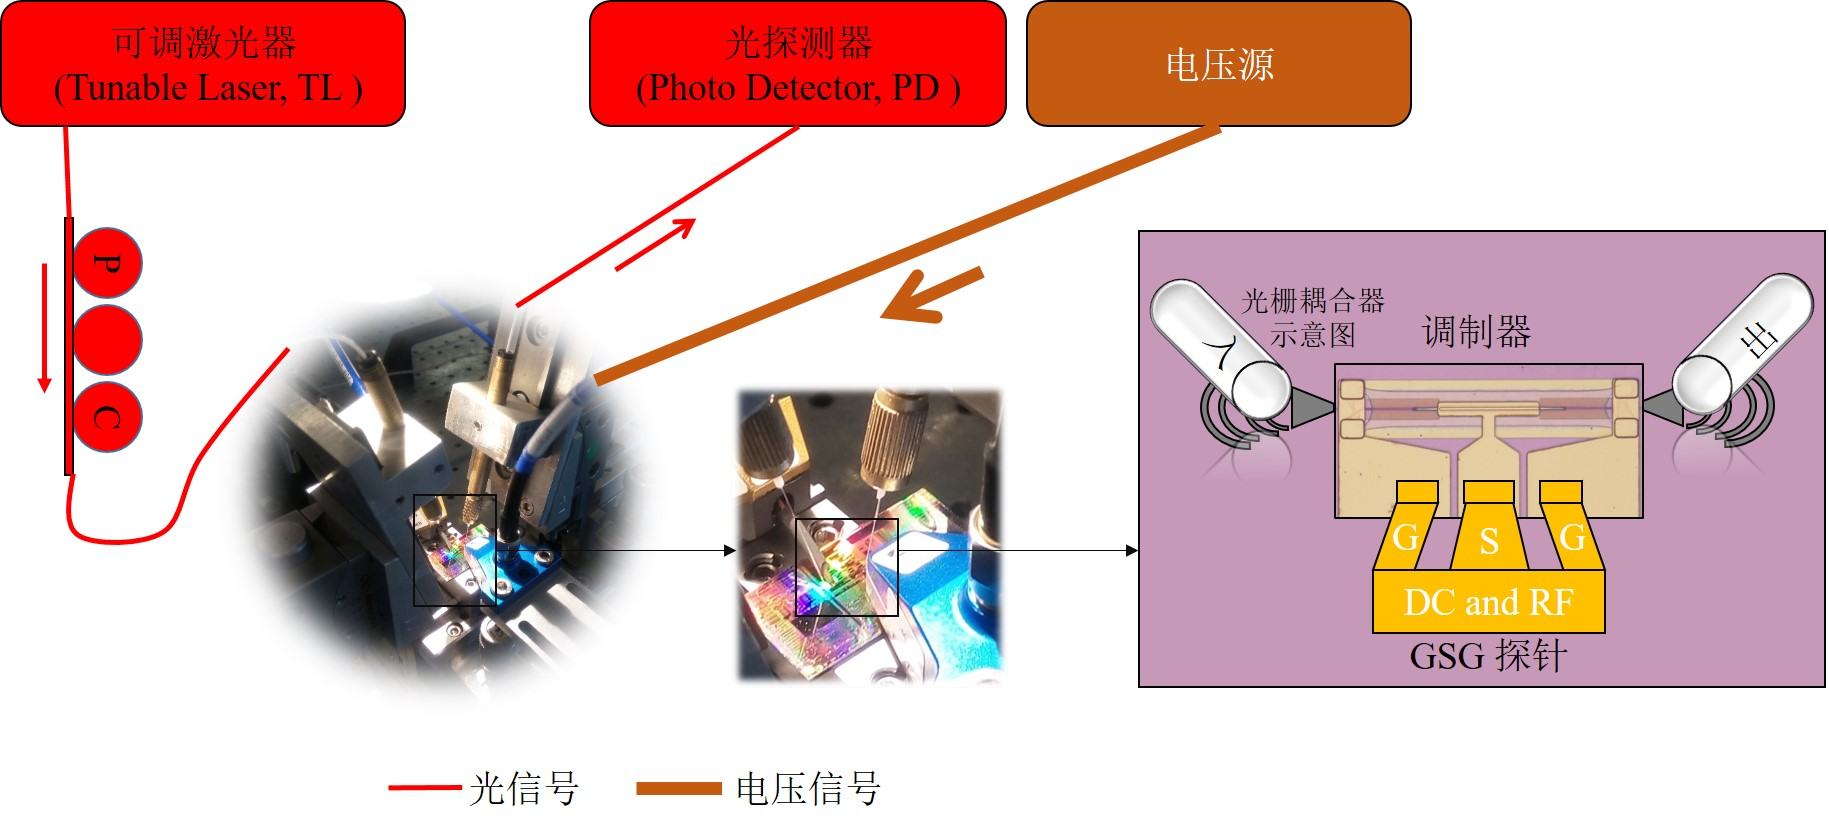
\includegraphics[width=15cm]{./Pictures/chapt4_static_measure_setup.jpg}
	\caption{硅基混合集成III-V电吸收光调制器的静态测试装置示意图,包含全局和局部示意图}
	\label{chapt4_static_measure_setup}
\end{figure}
我们构建的静态测试装置的结构示意图如图\ref{chapt4_static_measure_setup}所示。 其中,来自电压源的偏压通过同轴电缆连接到探针上,再与调制器上的GSG电极接触,将电信号直接加载到调制器上。而来自可调激光器的光信号,然后经过偏振控制器(Polarization Controller, PC),通过与垂直面成10$^\circ$角的光纤入射到硅基芯片上的耦合光栅上。耦合光栅用于将光纤中的光模式转化到硅波导中的光模式。光经过调制器,然后传播到输出耦合光栅上,再耦合回光纤光模式。最后,我们从光探测器读取光功率值。通过扫描电压源的偏压,我们就能获得调制器的静态响应,如图\ref{chapt4_static_measure_1550}所示。
\begin{figure}[htb]
	\centering
	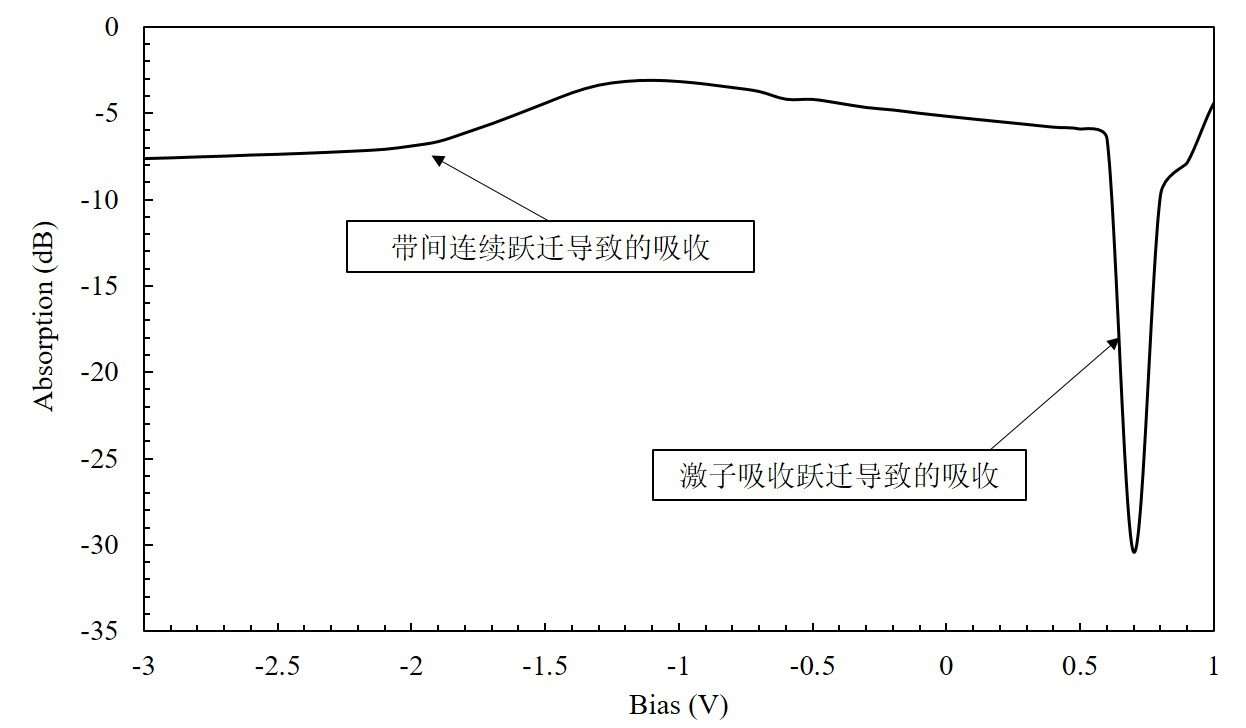
\includegraphics[width=14cm]{./Pictures/chapt4_static_measure_1550.jpg}
	\caption{调制区域80~$\mu m$长的硅基混合集成III-V电吸收光调制器,在不同偏压下对波长1.55 $\mu m$光的吸收变化曲线}
	\label{chapt4_static_measure_1550}
\end{figure}

图\ref{chapt4_static_measure_1550}中测试的调制器随电压的吸收曲线,已经减去直波导加上两个耦合光栅的损耗。可以看到在0~V偏压下调制器的插入损耗达到了5~dB,大于之前的仿真结果。这主要是由于MQW层和SCH层的实际宽度(见图\ref{chapt4_III_V_results}(a) )大于设计值1.5~$\mu m$ (见图\ref{chapt4_structure_mode_profile}(a) )。这意味着MQW层和SCH层的锥形尖端展宽,不仅激发出高阶模式,也增加了反射,导致耦合效率降低。从图\ref{chapt4_taper_performance}(d) 也可以看出,MQW层和SCH层的锥形尖端宽度增加会导致耦合效率的急剧降低。

图\ref{chapt4_static_measure_1550}中也展示了随着电压变化,调制器吸收谱有两段变化趋势。在反向偏压时,调制器的吸收的变化是由于带间连续跃迁随电压变化导致的。可以看到,80$\mu m$长的器件,在电压从-1~V变化到-2~V时,消光比只有4~dB的变化。当在正向偏压时,吸收的变化是由激子跃迁随电压变化导致的。同样长度的器件,在100~mV的电压变化下,就有大于20~dB消光比的变化。

\begin{figure}[htb]
	\centering
	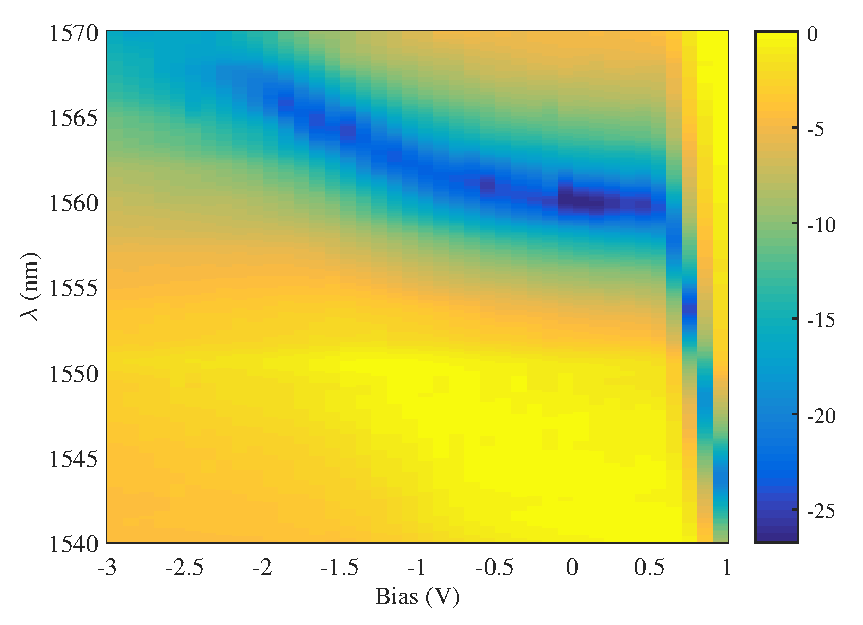
\includegraphics[width=14cm]{./Pictures/chapt4_static_measure_absorption_spectra.eps}
	\caption{调制区域80~$\mu m$长的硅基混合集成III-V电吸收光调制器,在不同偏压下的吸收谱的变化。可以看到,在正偏的情况下,激子吸收强度达到了20dB}
	\label{chapt4_static_measure_absorption_spectra}
\end{figure}
在图\ref{chapt4_static_measure_absorption_spectra}展示了,调制器的吸收谱随偏压的变化。激子的吸收峰随电压的实验和理论的预测值很好的吻合,如图\ref{chapt4_bandfilling_sim}所示。在正向偏压下,激子吸收峰随电压增加的蓝移速度达到了50~nm/V,并且激子吸收峰的强度一直保持着。因此,我们可以在正向偏压下,获得低驱动电压的电吸收光调制器。

\subsection{动态性能}
\begin{figure}[htb]
	\centering
	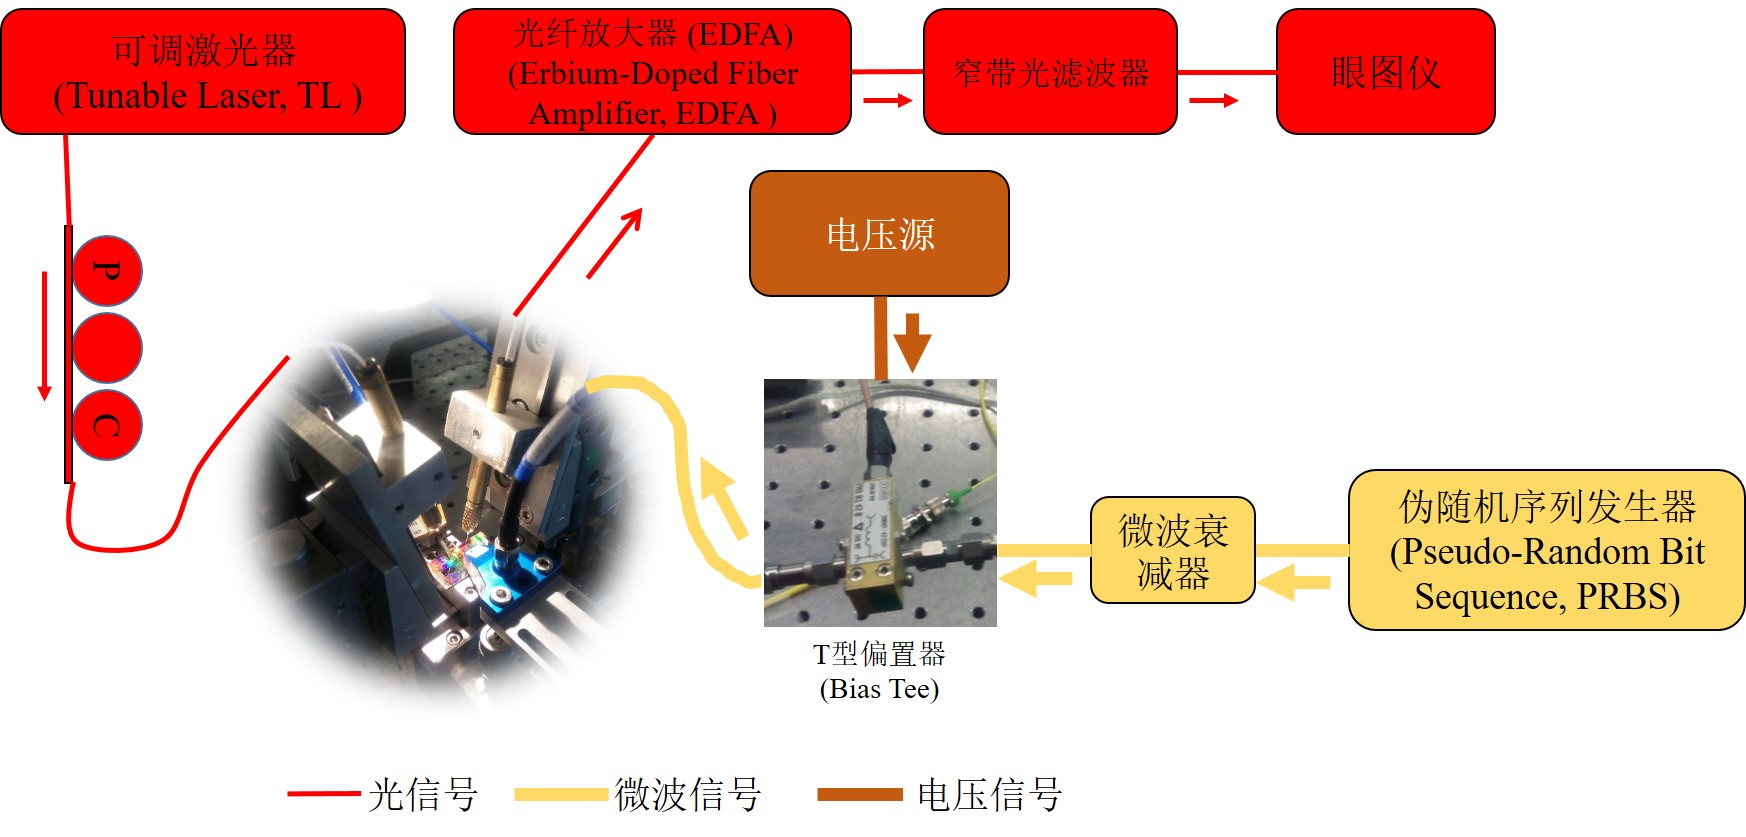
\includegraphics[width=15cm]{./Pictures/chapt4_dynamic_measure_setup.jpg}
	\caption{硅基混合集成III-V电吸收光调制器的动态眼图测试装置示意图}
	\label{chapt4_dynamic_measure_setup}
\end{figure}
\begin{figure}[htb]
	\centering
	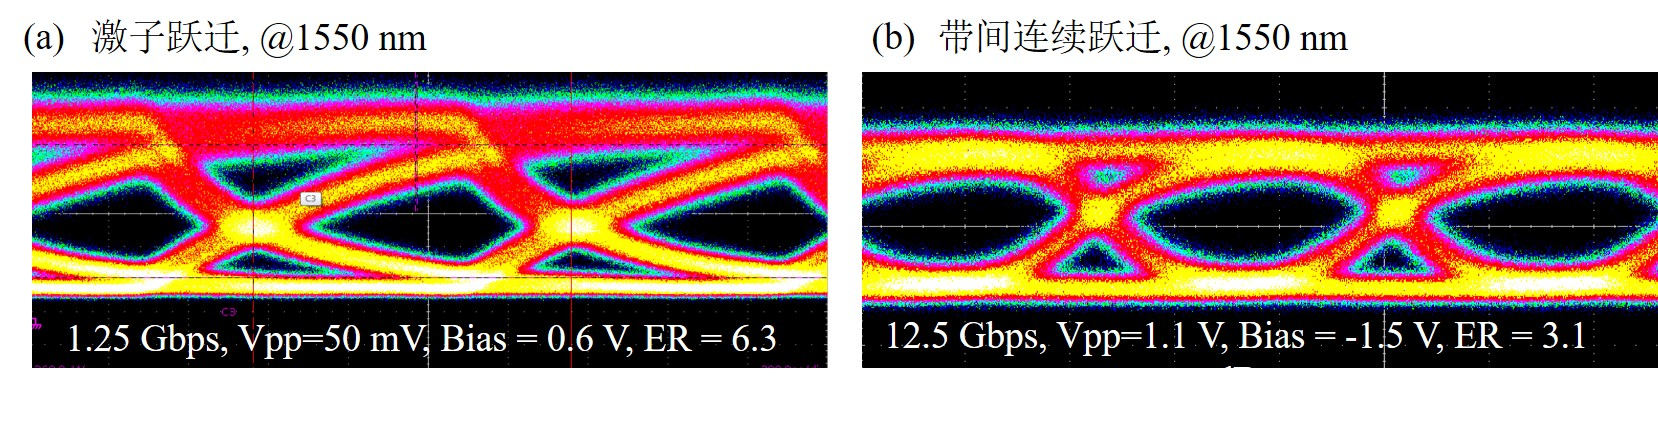
\includegraphics[width=15cm]{./Pictures/chapt4_eyediagram.jpg}
	\caption{硅基混合集成III-V电吸收光调制器在1.55~$\mu m$处,长度为2\SP{31}-1的PRBS NRZ眼图:(a) 正向偏压 0.6~V,1.25~Gbps时;(b)反向偏压-1.5~V,12.5~Gbps时}
	\label{chapt4_eyediagram}
\end{figure}
接下来我们测试电吸收光调制器在1.55~$\mu m$的动态特性。我们构建的动态测试装置的构建示意图如图\ref{chapt4_dynamic_measure_setup}所示。我们用伪随机二进制序列发生器(Pseudo-Random Bit Sequence, PRBS)产生长度为2\SP{31}-1的非归零码(Non-Return-to-Zero, NRZ)。然后进过微波衰减器将微波信号衰减到峰峰值为50~mV。再利用T型偏置器(Bias-Tee)将微波信号和静态偏压0.6~V耦合到同一条cable中,传输到GSG探针,加载到硅基混合集成III-V电吸收光调制器上。调制后的光从耦合光栅输出到光纤中。光纤中的光经过掺铒光纤放大器(Erbium-Doped Fiber Amplifier, EDFA)放大,再经过窄带光滤波器将EDFA的受激自发辐射谱滤除,输入到眼图仪中。图\ref{chapt4_eyediagram}(a)展示了1.25~Gbps的调制器眼图。动态的消光比达到了6.3~dB。相对于目前驱动电压最低的硅基光调制器,在相同的驱动电压下,基于能带填充效应的调制器消光比达到了它们的两倍。

调制器的功耗计算我们利用公式\ref{Equ:EC},根据我们之前100~$\mu m$长的调制器的电容值\cite{fu20155},估计我们调制器的结区电容大概116~fF。对应的动态调制器能耗是0.29~fJ/bit。动态调制能耗可以通过将MQW层和SCH宽度减小,进一步降低结区电容实现。调制器在1.25~Gbps的静态偏置能耗是110~fJ/bit。静态偏置能耗可以通过提高调制器的速度减小。值的注意的是,目前在正向偏压下,调制器的上升沿和下降沿的时间是受到量子阱中载流子的寿命限制。

图\ref{chapt4_eyediagram}(b)展示了调制器工作在反向-1.5~V的偏置电压,驱动电压的峰峰值为1.1~V时,12.5~Gbps的眼图。表面,我们可以在反偏下,使载流子寿命降低,提高调制速度。此时电吸收光调制器的速度受到RC常数的限制。利用调制掺杂的多量子阱结构,我们可以将电子的准费米能级在无偏压下提高到导带最低束缚能级之上,从而我们将正常工作点移动到反向偏压区域\cite{livescu1988free,kalinovsky1993free}。利用这种方法,基于能带填充效应的电吸收光调制器的调制速度将得到大幅度的提高。

\section{硅基混合集成III-V电吸收光调制器的双工作模式}
电吸收光调制器在反偏电压吸收光信号的同时,将光信号转化成了光电流。因此电吸收光调制器本身就是一个光探测器。下面我们将分析电吸收光调制器双工作模式中光探测器的静态和动态性能。最后,利用光调制器这一特性,实现了单片集成的光收发模块。
\subsection{光探测器的静态性能}
\begin{figure}[htb]
	\centering
	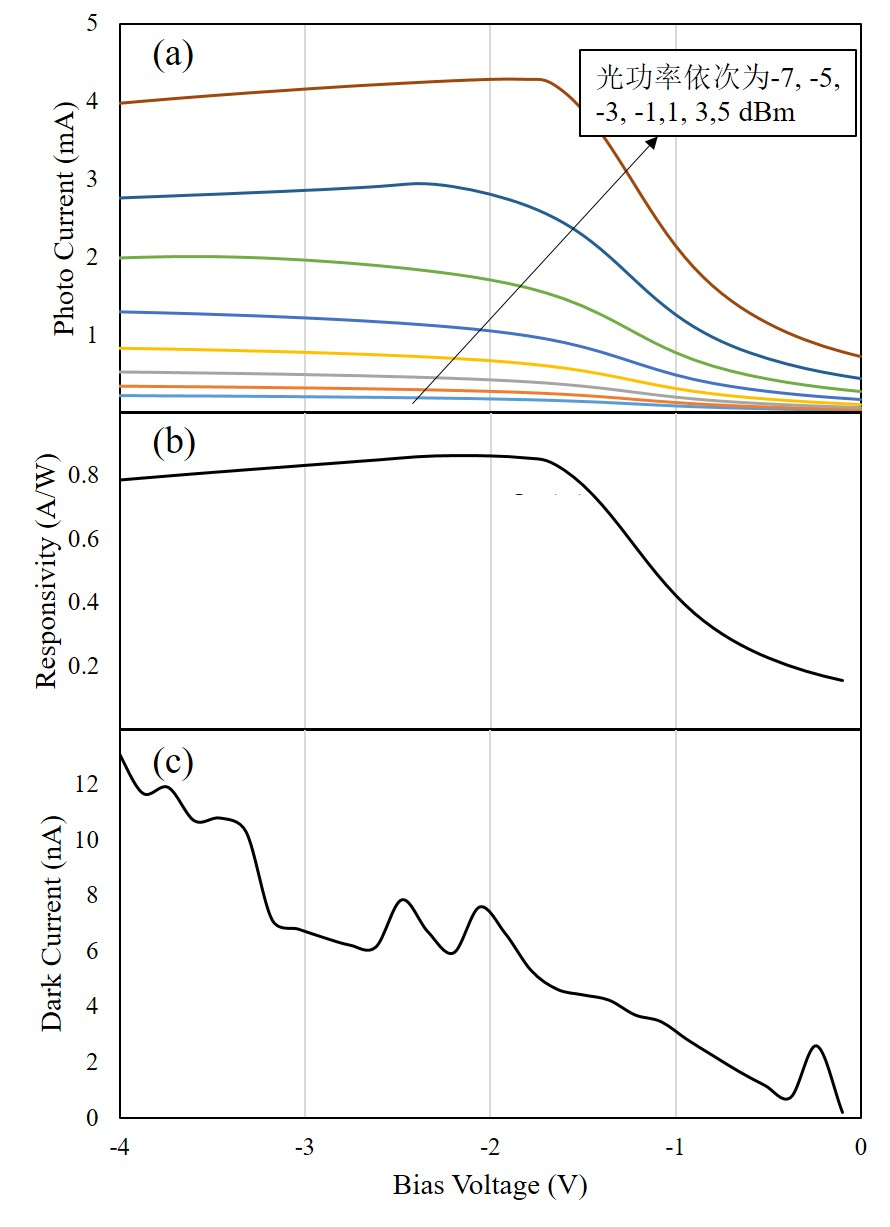
\includegraphics[width=12cm]{./Pictures/chapt4_pd_static.jpg}
	\caption{硅基混合集成III-V电吸收光调制器双工作模式下的光探测性能在1548~$n m$处(a) 不同输入光强下,反向偏压和光电流的关系;(b)反向偏压和光响应度的关系;(c)暗电流随反向电压的变化曲线}
	\label{chapt4_pd_static}
\end{figure}
我们构建的静态测试光探测器装置与图\ref{chapt4_static_measure_setup}相同。不过,我们不需要获取光纤的输出光强,只需要记录电压源上的光电流信号即可。图\ref{chapt4_pd_static}(a)展示了在波长1548~nm,不同偏压,不同输入光强下的光电流变化。可以看到当电压缓慢增大时,光电流先增大。当偏压达到-2~V时,光电流达到最大值,然后缓慢下降。对于不同光强,光电流一直是递增状态。图\ref{chapt4_pd_static}(b)根据输入光强和光电流的线性关系,我们拟合获得光探测器的响应度。可以看到,当偏压从-0.1~V达到-2~V时,对应的光响应度从0.15~A/W增大到了0.86~A/W。继续增加反偏电压到-4~V,光电流只是微弱减小到0.79~A/W。而暗电流随电压的变化如图\ref{chapt4_pd_static}(c)。可以看到当偏压从0~V变化到-4~V时,除了由于测试原因造成的抖动,暗电流单调递增到13~nA。 因此,电吸收光调制器作为光探测器也具有暗电流小,响应度大的特点。

\subsection{光探测器的动态性能}
\begin{figure}[htb]
	\centering
	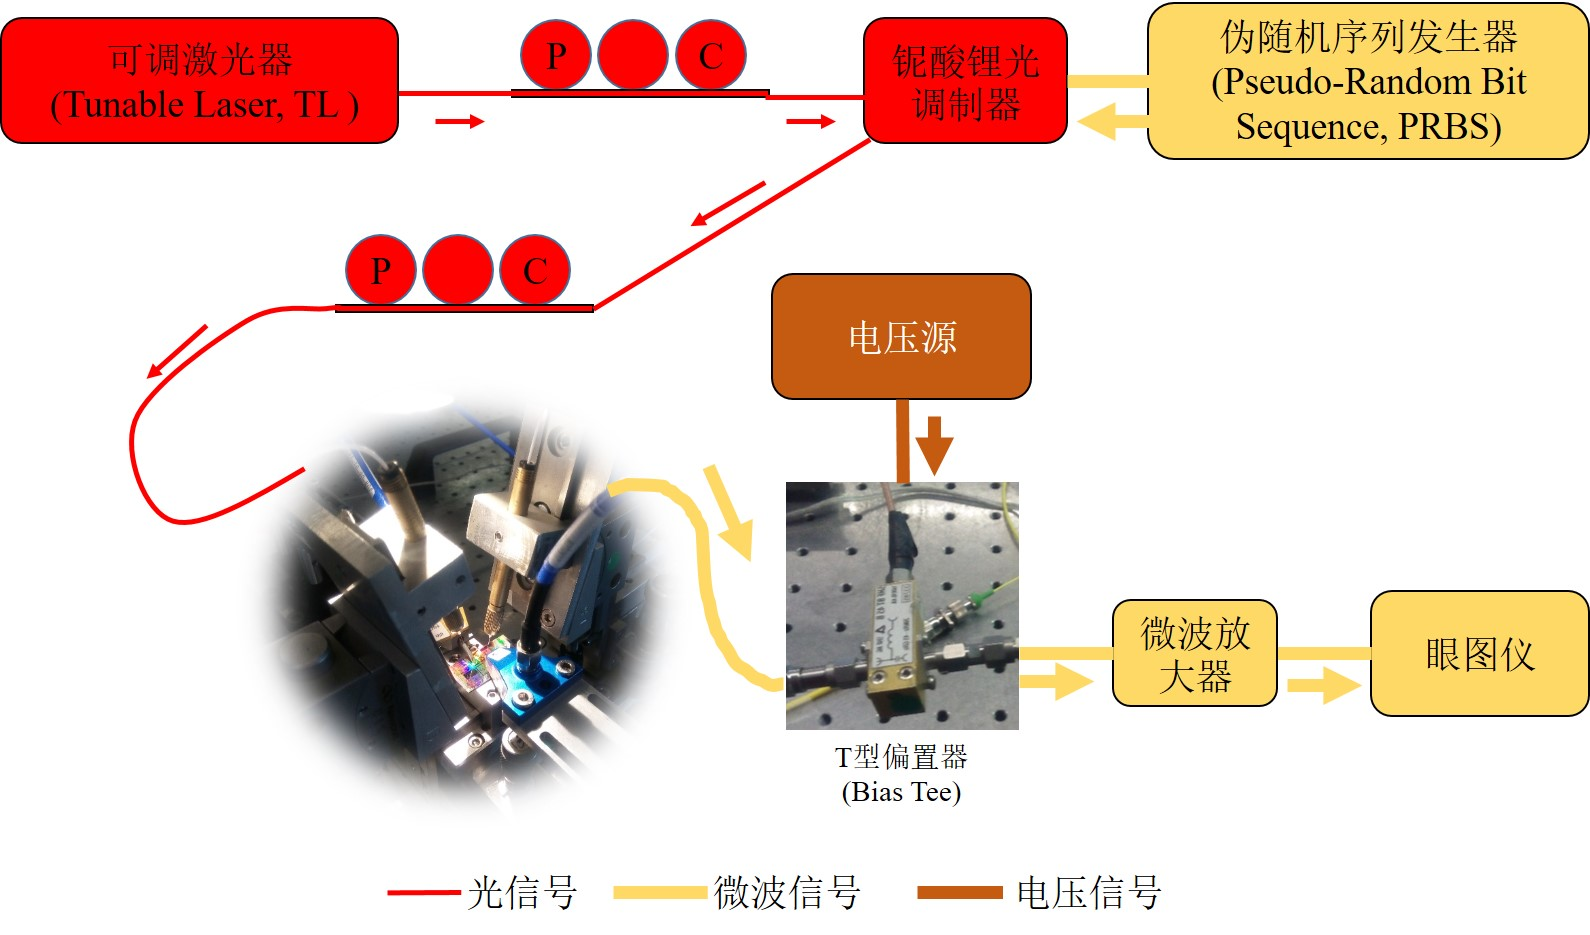
\includegraphics[width=15cm]{./Pictures/chapt4_dynamic_measure_setup_pd.jpg}
	\caption{硅基混合集成III-V电吸收光调制器用于光探测器时的动态眼图测试装置示意图}
	\label{chapt4_dynamic_measure_setup_pd}
\end{figure}
\begin{figure}[htb]
	\centering
	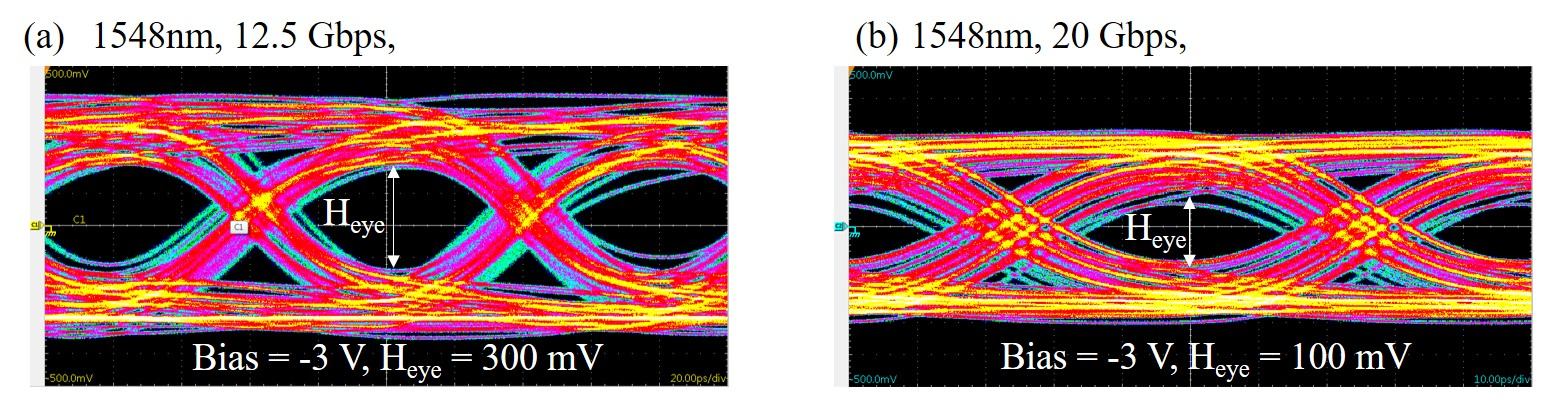
\includegraphics[width=15cm]{./Pictures/chapt4_eyediagram_pd.jpg}
	\caption{光探测器在1548~nm处,长度为2\SP{31}-1的PRBS NRZ眼图:(a)速度为12.5~Gbps时;(b)速度为20~Gbps}
	\label{chapt4_eyediagram_pd}
\end{figure}

接下来我们测试电吸收光调制器做为光探测器在1548~nm的动态特性。我们构建的动态测试装置的构建示意图如图\ref{chapt4_dynamic_measure_setup_pd}所示。我们用伪随机二进制序列发生器产生长度为2\SP{31}-1的非归零码,驱动商用的铌酸锂光调制器。铌酸锂光调制器将电信号再加载到从可调激光器输出,经过偏振控制器调节的光信号上。然后被调制器的光信号经过再偏振控制器通过耦合光栅耦合到硅波导中。偏置电压利用T型偏置器,将反向偏压-3~V加载到电吸收光调制器上。当被调制的光信号被电吸收光调制器吸收,就会转化成调制的光电流。这个调制器的光电流信号就会通过T型偏置器,滤除直流部分,经过微波放大器,传输到眼图仪中。

图\ref{chapt4_eyediagram_pd}(a)展示了光探测器探测得到的12.5~Gbps的眼图,眼图中间的高度$H_{eye}$有300~mV。这意味电吸收光调制器作为光探测器,也可以用于高速测试。不过光探测器的速度除了受到RC常数的限制外,还受到光生载流子从量子阱中迁移到电极所需的时间的限制。因此,加大偏置电压,能提高载流子的迁移速度。这也是我们不将偏压定于拥有最高光响应度的-2~V,而是选在-3~V的原因。当我们进一步将调制速率提高到20~Gbps时,探测器将光信号转化为电信号后的眼图如图\ref{chapt4_eyediagram_pd}(b)所示。眼睛中间的高度降低到了100~mV。

\subsection{单片集成的光收发模块}
单片集成的光收发模块,充分利用了硅基混合集成III-V平台的三个优点,第一个是硅基平台紧凑的无源光波导器件;第二个是III-V电吸收光调制器的双工作模式;第三个是能带填充效应使电吸收光调制器具有大的消光比。
\begin{figure}[htb]
	\centering
	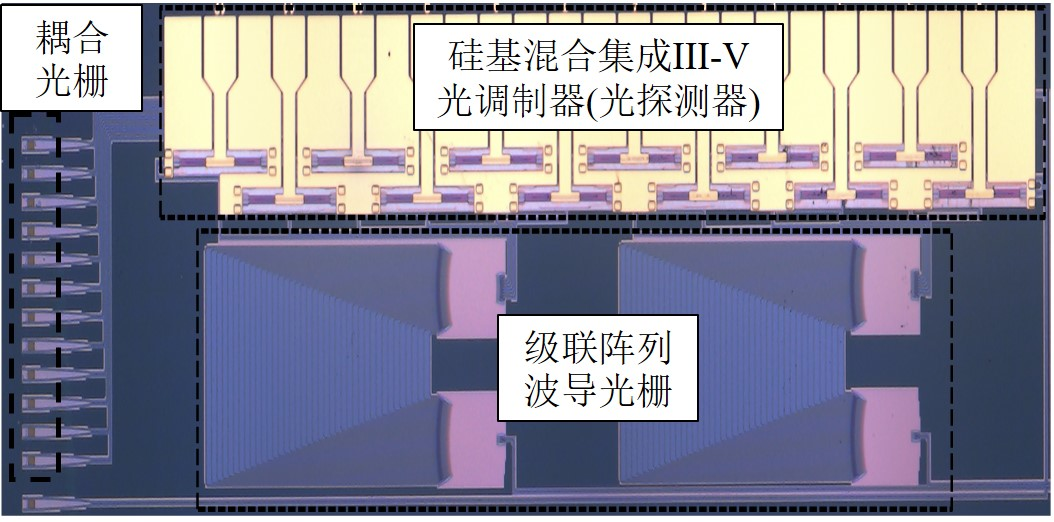
\includegraphics[width=12cm]{./Pictures/chapt4_casacade_awg_structure.jpg}
	\caption{单片集成6通道双级联阵列波导光栅的光收发模块显微镜俯视图。整个器件的尺寸3$\times$0.65 mm\SP{2}}
	\label{chapt4_casacade_awg_structure}
\end{figure}
\begin{figure}[htb]
	\centering
	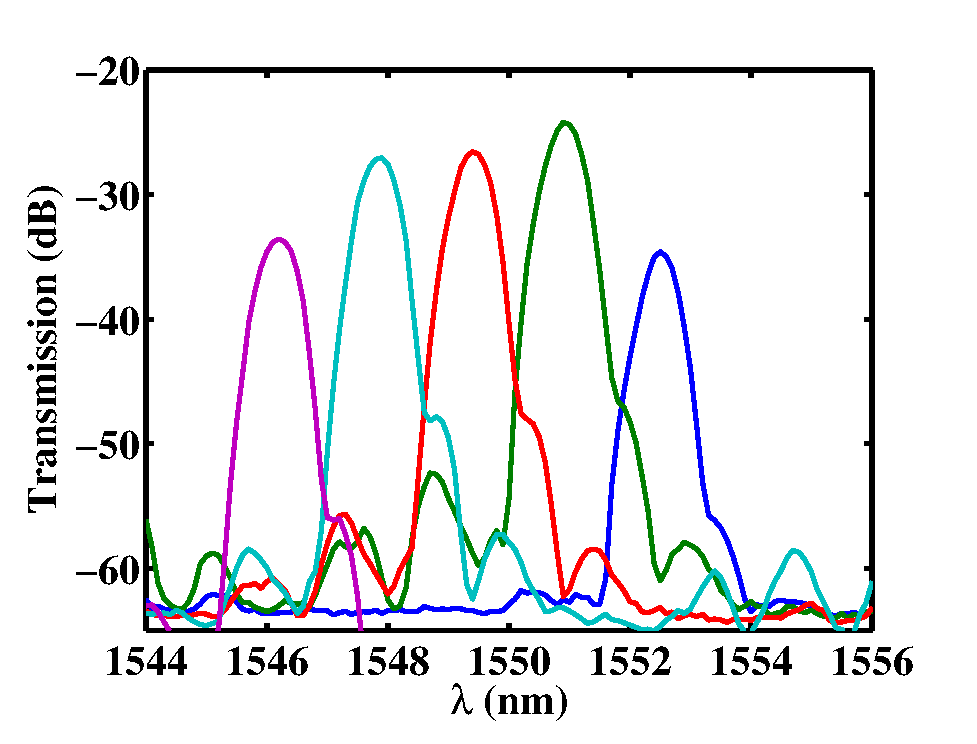
\includegraphics[width=12cm]{./Pictures/chapt4_cascade_awg_spectra.eps}
	\caption{级联阵列波导光栅的光谱图(其中一个通道损坏)}
	\label{chapt4_cascade_awg_spectra}
\end{figure}

借助于硅基平台紧凑的无源光波导器件,我们实现了在3$\times$0.65~mm\SP{2}的面积内集成了两个级联的6通道,通道间隔1.6~nm的阵列波导光栅(Arrayed Waveguide Grating, AWG),6个硅基混合集成III-V光调制器和6个同样结构的光探测器。图\ref{chapt4_casacade_awg_structure}展示了器件的俯视图。图\ref{chapt4_cascade_awg_spectra}展示了集成调制器的阵列波导光栅的光谱图。

借助于电吸收光调制器的双工作模式,我们将6个调制器和1个AWG构成一个波长复用的光发射端,另外一边1个AWG和6个光探测器构成一个波长解复用的光接收端。由于发射端和接收端的结构相同,我们直接级联就实现了基于波长复用的单片集成的光收发模块。

借助于能带填充效应的高消光比特性,提高了调制器输出信号的信噪比,从而克服了级联AWG中大的插入损耗导致探测器的信号被噪声淹没信号的问题。帮助我们在接收端观察到了睁开的眼图。

\begin{figure}[htb]
	\centering
	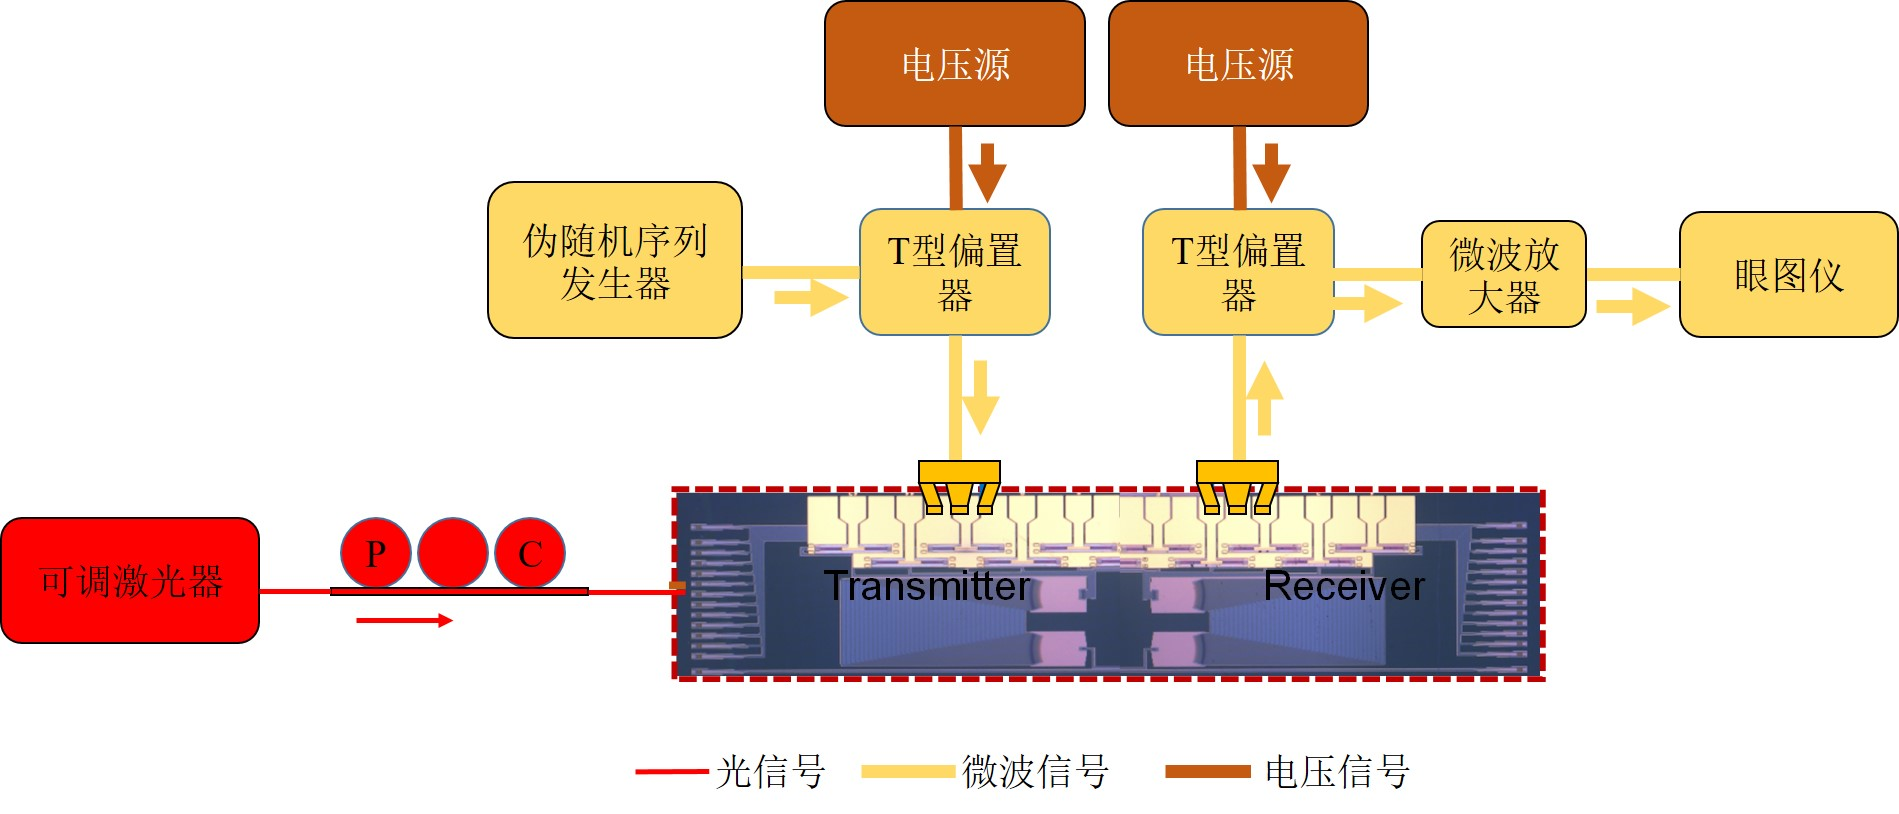
\includegraphics[width=15cm]{./Pictures/chapt4_tranciever_measure.jpg}
	\caption{光收发模块的测试装置示意图}
	\label{chapt4_tranciever_measure}
\end{figure}

\begin{figure}[htb]
	\centering
	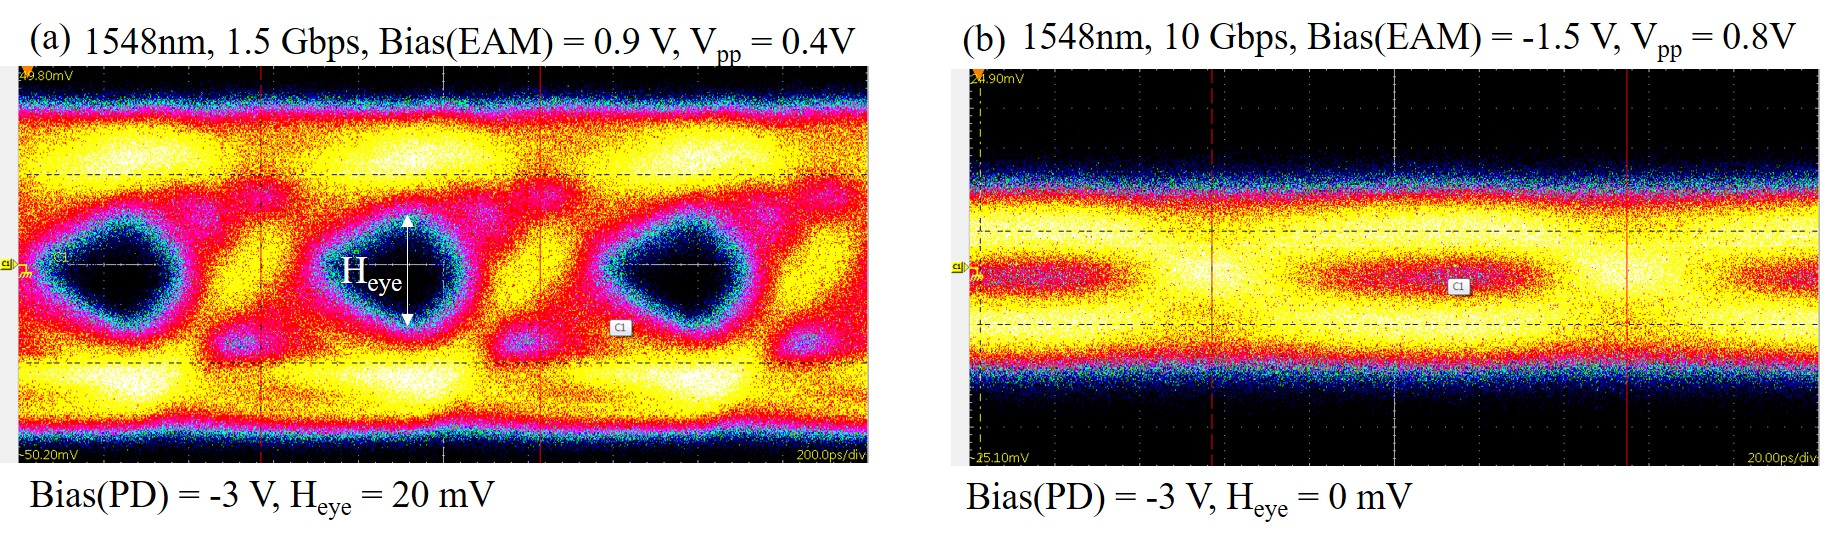
\includegraphics[width=15cm]{./Pictures/chapt4_cascade_eyediagram.jpg}
	\caption{1548~nm级联通道的眼图,长度为2\SP{31}-1的PRBS NRZ眼图:(a) 正向偏压 0.9~V,1.5~Gbps时;(b)反向偏压-1.5~V,10~Gbps时}
	\label{chapt4_cascade_eyediagram}
\end{figure}

光收发模块的测试装置图,如图\ref{chapt4_tranciever_measure}所示。可调激光器输出的光信号首先经过偏振控制器,再经过光栅耦合器传播到硅波导中。在发射端,通过T型偏置器,我们将PRBS产生长度为2\SP{31}-1的NRZ与偏置电压加载到调制器上。被光调制器调制后的光信号,经过两个级联的AWG传播到光探测器。光探测器由电压源连接第二个T型偏置器,给予偏置电压。光探测器产生的光电流,经过T型偏置器,滤除直流部分,被微波放大器放大后传播到眼图上。图\ref{chapt4_cascade_eyediagram}(a)给出了一个插入损耗比较小的级联通道的眼图。我们可以观测到睁开的眼图,不过眼睛$H_{eye}$高度只有20~mV。这是由于级联AWG的插入损耗达到了24~dB。这意味着从调制器出来,只有0.4\%的光耦合到光探测器中。如果,我们将调制器工作在反向偏置电压下,由于光调制器的消光比只有3~dB,我们在接收端就无法观察到睁开的眼睛,如图\ref{chapt4_cascade_eyediagram}(b)所示。

在此,我们初步实现了基于波长复用的单片硅衬底上的光收发模块,观察到了睁开的眼图。不过,为了进一步优化单片集成的光收发模块,我们发现有三个方面需要改进。首先需要降低目前硅基平台上AWG等无源器件和混合集成III-V光调制器、光探测器的插入损耗。其次需要一个高速,高消光比的光调制器。最后,需要在硅基上集成光放大器,从而弥补因器件增加而导致的额外损耗。

\section{本章小结}
在本章中,我们首先介绍了基于能带填充效应的低驱动电压的电吸收光调制器的工作原理。然后,我们对调制器的波导结构,硅波导与硅基混合集成III-V波导的耦合结构,电极结构,能带结构进行了设计和仿真。其中,我们首次仿真了综合QCSE效应和能带填充效应的激子吸收峰随外界电压变化的漂移图。仿真结果与器件的静态测试结果相吻合。接着,我们先简要介绍了硅波导的两种加工方式,再详细介绍了制作硅基混合集成III-V电吸收光调制器的键合工艺和III-V波导的加工步骤。我们利用III-V材料选择性腐蚀的特点,摸索出了全湿法制作混合集成III-V波导的新工艺流程,简化了工艺步骤。在加工结束后,我们介绍了用于降低金属和半导体接触电阻的电压快速退火法。随后,在搭建的测试光调制器的高速平台上,对其高速性能进行了测试。我们制作的基于能带填充效应的光调制器,驱动电压只需要50~mV,动态消光比有6.3~dB,速度能达到1.25~Gbps。目前,调制速度主要受到载流子寿命的影响。通过对量子阱区域进行掺杂,使调制器工作在反向偏压,能进一步提高调制速度。

接下来,我们对电吸收光调制器作为光探测器的静态和动态性能进行了测试。我们验证了电吸收调制器本身就可以作为高速光探测器。探测速度可以达到20~Gbps,在-2~V偏压下的响应度为0.86~A/W。最后,借助于硅基平台,我们初步实现了单片混合集成阵列波导光栅,高速调制器,高速探测器的的光收发模块。而电吸收光调制器的双工作模式和能带填充效应下的高消光比,使我们克服了光路中的高插入损耗,在探测器中观测到了睁开的眼图。
